\documentclass[a4paper]{article}

\usepackage{isapreamble}

\title{\huge \textbf{MA E\(\chi\) 02}}
\author{
  isagila
  \and
  \href{https://t.me/pochtineploho}{@pochtineploho}
  \and
  \href{https://t.me/DUBSTEPHAVEGUN}{@DUBSTEPHAVEGUN}
}
\date{Собрано {\ddmmyyyydate\today} в \currenttime}
\titlepic{\includegraphics[width = \textwidth]{misc/title.png}}

\begin{document}

%% Отступы перед/после формул
\setlength{\abovedisplayskip}{-5pt}
\setlength{\abovedisplayshortskip}{0pt}
\setlength{\belowdisplayskip}{0pt}
\setlength{\belowdisplayshortskip}{0pt}

\clearpage
\maketitle
\thispagestyle{mainpage}
\newpage
\setcounter{page}{2}
\tableofcontents

\newpage
\section{Интегрирование функции одной переменной}

\begin{questions}
  \question{Обыкновенное дифференциальное уравнение (ДУ): задача о радиоактивном распаде и задача о падении тела. Определение ДУ, решения ДУ и их геометрический смысл. Задача Коши.}

\begin{definition}
  Обыкновенным ДУ\(_{n}\) называется

  \begin{align*}
    F(x, y, \dotsc, y^{(n)}) = 0
  \end{align*}
\end{definition}

\begin{remark}
  'Обыкновенное' означает не в частных дифференциалах, т.е. \(y(x)\) это
  функция одно переменной.
\end{remark}

\begin{definition}
  Порядком ДУ называется наивысший порядок входящей в него производной.
\end{definition}

\begin{definition}
  Решением ДУ\(_{n}\) является функция, которая обращает его в верное равенство.
\end{definition}

\begin{definition}
  Кривые, соответствующие решениям ДУ называются интегральными кривыми.
\end{definition}

\begin{definition}
  Если решение ДУ задано неявно \(\phi(x, y(x)) = 0\), то 
  \(\phi(x, y(x)) = 0\) называется интегралом ДУ.
\end{definition}

\begin{definition}
  Решение ДУ с неопределенными константами \(c_{i}\) называется общим решением
  (общим интегралом) ДУ.  
\end{definition}

\begin{definition}
  Решение ДУ с определенными константами \(c_{i}\) называется частным решением
  (частным интегралом) ДУ.
\end{definition} 

\begin{definition}
  Система из ДУ\(_{n}\) и \(n\) начальных условий вида

  \begin{align*}
    \begin{cases}
      \text{ДУ}_n \\
      y_0 = y(x_0) \\
      y'_0 = y'(x_0) \\
      \dots \\
      y^{(n - 1)}_0 = y^{(n - 1)}(x_0)
    \end{cases}
  \end{align*}

  называется задачей Коши. \(n\) начальных условий необходимы для определения
  \(n\) констант \(c_{i}\).
\end{definition}

\begin{remark}
  Подробнее про задачу Коши и геометрический смысл решений рассказано в
  \ref{ex-un-Cp}.
\end{remark}

\underline{Задача о радиоактивном распаде}: 

Пусть есть \(Q\) грамма урана, скорость распада которого зависит от его массы с
некоторым коэффициентом \(k\). Требуется вывести формулу для подсчета массы
урана в момент времени \(t\).

Составим ДУ и решим его:

\begin{align*}
  \frac{\dd Q}{\dd t} = -k Q \mid \colon Q \neq 0
  \\
  \frac{\dd Q}{Q \dd t} = -k
  \iff
  \frac{\dd \ln Q}{\dd t} + k = 0
  \\
  \frac{\dd \ln Q + k \dd t}{\dd t} = 0
  \iff
  \frac{\dd (\ln Q + k t)}{\dd t} = 0
  \\
  \ln Q + kt = c_{1} \\
  Q = \widehat{c_{1}} e^{-k t}
\end{align*}

Из полученных интегральных кривых выбираем одну, которая соответствует
заданным начальным условиям.

\underline{Задача о падении тела}: 

Тело свободно падает вниз с заданной начальной скоростью. Требуется вывести
закон движения (закон изменения координат с течением времени).

Составим ДУ и решим его:

\begin{align*}
  \vec{F} = m \vec{a} = m \vec{g} \implies a = y''(t) = g \\
  \frac{\dd^{2} y(t)}{\dd t^{2}} = g
  \implies \frac{\dd v(t)}{\dd t} = g 
  \implies v(t) = g t + c_{1} \\
  \frac{\dd y(t)}{\dd t}  = v(t) = g t + c_{1}
  \implies y(t) = \frac{g t^{2}}{2} + c_{1} t + c_{2}
\end{align*}

Как и в первой задаче здесь получено общее решение. Константы можно найти
подстановкой начальных условий.

  \question{Замена переменной в неопределенном интеграле. Интегрирование по частям.}

\begin{remark}
  Интеграл сохраняет инвариантность своей формы, т.е.

  \begin{align*}
    \int f(\clubsuit) \dd \clubsuit = F(\clubsuit) + C
  \end{align*}
\end{remark}

\begin{theorem}\label{ad-rep}
  О замене производной в неопределенном интеграле

  Если \(x = \phi(t)\), где \(\phi(t)\) обратимая и дифференцируемая
  функция, то

  \begin{align*}
    \int f(x) \dd x = \int f(\phi(t)) \phi'(t) \dd t
  \end{align*}
\end{theorem}
\begin{proof}
  Возьмем производные от обоих частей:

  \begin{align*}
    \left( \int f(x) \dd x \right)'_{x} = f(x) \\
    \left( \int f(\phi(t)) \phi'(t) \dd t \right)'_{x} =
    \left( \int f(\phi(t)) \phi'(t) \dd t \right)'_{t} \frac{\dd t}{\dd x}
    \transition{\ref{ad-prop-2}}
    f(\phi(t)) \phi'(t) \frac{\dd t}{\dd x} =
    f(\phi(t)) \phi'(t) \frac{1}{\phi'(t)} =
    f(\phi(t)) =
    f(x)
  \end{align*}
\end{proof}

\begin{remark}
  Формула работает в обе стороны:

  \begin{align*}
    \int \frac{e^{\sqrt{x}}}{\sqrt{x}} \dd x
    \transition{\sqrt{x} = t}
    \int \frac{e^{t}}{t} 2t \dd t =
    2 e^{t} + C =
    2 e^{\sqrt{x}} + C
  \end{align*}

  \begin{align*}
    \int e^{x^{2}} \underbrace{2x \dd x}_{\dd x^2}
    \transition{x^2 = t}
    \int e^{t} \dd t =
    e^{t} + C =
    e^{x^2} + C
  \end{align*}
\end{remark}

\begin{theorem}
  Интегрирование по частям

  \begin{align*}
    \int u \dd v = u v - \int v \dd u
  \end{align*}
\end{theorem}
\begin{proof}
  Рассмотрим равенство \((u v)' = u' v + u v'\) и проинтегрируем обе его части:

  \begin{align*}
    (u v)' = u' v + u v'
    \\
    \int (u v)' \dd x = \int u' v + u v' \dd x
    \\
    u v = \int u' v \dd x + \int u v' \dd x
      \tag*{Линейность интеграла (\ref{ad-prop-3})}
    \\
    u v = \int v \dd u + \int u \dd v
      \tag*{Внесение под дифференциал (\ref{ad-rep})}
    \\
    \int u \dd v = u v - \int u \dd v
  \end{align*}
\end{proof}

\begin{remark}
  Интегрирование по частям используется если \(\int v \dd u\) вычисляется проще,
  чем интеграл \(\int u \dd v\). В качестве функции \(u\) выбирают ту, которая
  упрощается при дифференцировании.
\end{remark}

  \question{Детерминированный конечный автомат.}

Детерминированный конечный автомат (ДКА) это кортеж вида
\(\Tuple{\Sigma, Q, q_{0}, F, \delta}\), где
\begin{itemize}
  \item \(\Sigma\) это алфавит
  \item \(Q\) это множество состояний
  \item \(q_{0}\) это начальное состояние (\(q_{0} \in Q\))
  \item \(F\) это множество принимающих состояний (\(F \subseteq Q\))
  \item \(\delta\) это функция перехода \(\delta \colon Q \times \Sigma \to Q\)
\end{itemize}

Мы рассматриваем только автоматы-детекторы, т.е. им на вход подается слово,
после обработки которого автомат оказывается в одном из состояний. Если это
принимающее состояние, то говорят, что слово принимается автоматом (автомат
допускает слово), в противном случае~--- слово отвергается автоматом.

\underline{Вычисление}:

\begin{definition}
  Снимок (\textit{snapshot}) это упорядоченная пара вида \(\Pair{q, s}\), где
  \(q \in Q\) это текущее состояние, а \(s\) это еще непросмотренная часть входной
  строки.
\end{definition}

Множество всех снимков обозначается \(SNAP\). На этом множество можно ввести
бинарное отношение \(\vdash\), которое будет показывать, можно ли перейти от
одного снимка к другому:

\begin{align*}
  \Pair{q_{1}, s_{1}} \vdash \Pair{q_{2}, s_{2}}
  \iff
  \begin{cases}
    s_{1} = \alpha s_{2} \\
    \delta(q_{1}, \alpha) = q_{2}
  \end{cases}
\end{align*}

\begin{definition}
  Автоматный язык \(\Lang(\mathcal{A})\) это язык, состоящий из слов,
  принимаемых автоматом:

  \begin{align*}
    \Lang(\mathcal{A})
    = \{ s \mid \Pair{a_{0}, s} \vdash^{*} \Pair{f, \epsilon}, f \in F \}
  \end{align*}
\end{definition}

\begin{definition}
  Множество автоматных языков \(AUT\) это множество языков, для которых
  существует автомат их принимающий.

  \begin{align*}
    AUT = \{
      \mathcal{X} \mid \exists \mathcal{A} \colon
      \Lang(\mathcal{A}) = \mathcal{X}
    \}
  \end{align*}
\end{definition}

  \question{Композиции.}

\begin{definition}
  Слабой композицей числа \(n \ge 0\) на \(k\) частей называется решение
  уравнения \(b_{1} + \dotsc + b_{k} = n\) при условии \(b_{i} \ge 0\).
\end{definition}

Для подсчета числа слабых композиций воспользуемся методом Stars\&Bars: пусть у
нас есть \(n\) единиц и \(k - 1\) перегородка между ними, значит всего получаем

\begin{align*}
  \Big|
    \text{Количество слабых композиций } n \text{ на } k \text{ частей}
  \Big|= \binom{n + k - 1}{k - 1}
\end{align*}

\begin{definition}
  Композицией числа \(n \ge 0\) на \(k\) частей называется решение уравнения
  \(b_{1} + \dotsc + b_{k} = n\) при условии \(b_{i} \ge 0\).
\end{definition}

Количество композиций числа можно посчитать следующим образом: возьмем из \(n\)
\(k\) единиц (по одной для каждого слагаемого), а для оставшихся \(n - k\)
единиц решим задачу о слабой композиции. Итого получим

\begin{align*}
  \Big|
    \text{Количество композиций } n \text{ на } k \text{ частей}
  \Big| = \binom{n - 1}{k - 1}
\end{align*}

\begin{remark}
  Число композиций числа \(n\) на произвольное число частей
  (т.е. \(k = 1 \dots n\)) равно \(2^{n - 1}\).
\end{remark}

  \subsection{%
  Предельный переход в неравенствах. Теорема о двух милиционерах.%
}

\begin{theorem} \label{thr:lim-func}
  Если функция \(f(x)\) имеет предел в точке \(a\), то она ограничена в
  некоторой проколотой окрестности этой точки.
\end{theorem}

\begin{proof}
  Раскроем модуль в определении предела.

  \begin{equation*}
    \begin{aligned}
      \lim_{x \to a} f(x) = L \iff
      \forall \epsilon > 0 \exists \delta > 0 \given
      \forall x \in \nearo{a}{\delta} \cap E \implies
      \abs{f(x) - L} < \epsilon
    \\
      L - \epsilon < f(x) < L + \epsilon
    \end{aligned}
  \end{equation*}

  Получается, что функция \(f(x)\) ограничена в проколотой окрестности точки
  \(a\).
\end{proof}

\begin{theorem}[О стабилизации знака] \label{thr:stable-sign}
  Если \(\lim_{x \to a} f(x) = A > 0\), то \(f(x) > 0\) в некоторой окрестности
  \(a\).
\end{theorem}

\begin{proof}
  По теореме \ref{thr:lim-func}, получаем, что \(f(x)\) ограничена в некоторой
  проколотой \(\epsilon\)--окрестности точки \(a\), т.е. \(A - \epsilon < f(x)
  < A + \epsilon\). Пусть \(\epsilon = \frac{A}{2}\), тогда \(f(x) > A -
  \frac{A}{2} > 0\).
\end{proof}

\begin{theorem}[О предельном переходе в неравенствах]
  Если \(f(x) \le g(x)\) в некоторой окрестности точки \(a\), то 
  
  \begin{equation*}
    \begin{rcases}
      \lim_{x \to a} f(x) = A \\
      \lim_{x \to a} g(x) = B
    \end{rcases}
    \implies
    A \le B
  \end{equation*}
\end{theorem}

\begin{proof}
  От противного: пусть \(A > B\), тогда

  \begin{equation*}
    \lim_{x \to a} f(x) - \lim_{x \to a} g(x)
    = \lim_{x \to a} (f(x) - g(x))
    = A - B > 0
  \end{equation*}

  Тогда по \ref{thr:stable-sign} \(f(x) - g(x) > 0\), т.е. \(f(x) > g(x)\) в
  некоторой проколотой \(\delta_1\)--окрестности точки \(a\). По условию \(f(x)
  \le g(x)\) в некоторой \(\delta_2\)-окрестности точки \(a\). Пусть \(\delta =
  \min(\delta_1, \delta_2)\), тогда по свойству окрестностей оба условия должны
  выполняться, т.е. \(f(x) \le g(x)\) и \(f(x) > g(x)\). Противоречие.
\end{proof}

\begin{theorem}[О двух милиционерах] \label{thr:squeezed-func}
  Если \(f(x) \le h(x) \le g(x)\) в некоторой проколотой окрестности точки
  \(a\), то

  \begin{equation*}
    \begin{rcases}
      \lim_{x \to a} f(x) = A \\
      \lim_{x \to a} g(x) = A
    \end{rcases}
    \implies
    \lim_{x \to a}h(x) = A
  \end{equation*}
\end{theorem}

\begin{proof}
  Запишем условие формально, раскрыв два предела по определению

  \begin{equation*}
    \begin{aligned}
      \lim_{x \to a} f(x)  = A \iff
      \forall \epsilon > 0 \exists \delta_1 > 0 \given
      \forall x \in \nearo{a}{\delta_1} \cap X \implies
      \abs{f(x) - A} < \epsilon
    \\
      \lim_{x \to a} g(x) = A \iff
      \forall \epsilon > 0 \exists \delta_2 > 0 \given
      \forall x \in \nearo{a}{\delta_2} \cap X \implies
      \abs{g(x) - A} < \epsilon
    \\
      \exists \delta_3 > 0 \given
      \forall x \in \nearo{a}{\delta_3} \cap X \colon
      f(x) \le h(x) \le g(x)
    \end{aligned}
  \end{equation*}

  Пусть \(\delta = \min(\delta_1, \delta_2, \delta_3)\), тогда по свойству
  окрестностей все условия будут выполняться. Раскроем модули по определению и
  \quote{склеим} полученные неравенства.

  \begin{equation*}
    \begin{rcases}
      A - \epsilon < f(x) < A + \epsilon \\
      A - \epsilon < g(x) < A + \epsilon
    \end{rcases}
    \implies
    A - \epsilon < f(x) \le h(x) \le g(x) < A + \epsilon
    \implies
    A - \epsilon < h(x) < A + \epsilon
  \end{equation*}

  Причем последнее неравенство выполняется в проколотой окрестности точки \(a\)
  для любого \(\epsilon\). Таким образом \(\lim_{x \to a} f(x) = A\) по
  определению предела.
\end{proof}

Теорема \ref{thr:squeezed-func} также называется теоремой о двух жандармах или
теоремой о сжатой функции.

  \question{Двудольные графы.}

\begin{definition}
  Двудольный граф это граф, вершины которого могут быть разбиты на два множества
  (две доли) так, что между вершинами каждого из множеств не будет ребер.
\end{definition}

\begin{remark}
  Об обозначениях.

  Двудольный граф обычно обозначается как \(G = \Triple{X, Y, E}\), где \(X\) и
  \(Y\) это его доли, а \(E\)~---- множество ребер между этими долями.

  Пусть задано некоторое подмножество \(S \subseteq X\), тогда \(E(S)\) это
  множество ребер, инцидентных вершинам из множества \(S\).

  Обозначение \(N(S)\) используется что показать 'соседей' для вершин из
  множества \(S\), т.е. такие вершины из множества \(Y\), которые смежны хотя
  бы с одной из вершин из множества \(S\).
\end{remark}

\begin{definition}
  Двудольный граф называется сбалансированным, если размеры его долей совпадают.
\end{definition}

\begin{theorem}\label{bipartite-balance}
  \(r\)-регулярный двудольный граф является сбалансированным.
\end{theorem}
\begin{proof}
  Пусть дан двудольный граф \(G = \Triple{X, Y, E}\).
  Т.к. он двудольный, то множество ребер может быть представлено в виде
  \(\abs{E} = \abs{X} \cdot r\). С другой стороны оно может быть представлено в
  виде \(\abs{E} = \abs{Y} \cdot r\). Приравниваем и получаем искомое равенство
  \(\abs{X} = \abs{Y}\).
\end{proof}

\begin{theorem}
  В любом регулярном двудольном графе существует совершенное паросочетание.
\end{theorem}
\begin{twocolumns}
  \begin{proof}
    Рассмотрим двудольный граф \(G = \Triple{X, Y, E}\). Выберем произвольное
    \(S \subseteq X\). Заметим, что \(E(N(S)) \ge E(S)\), причем т.к. граф
    регулярный, то \(E(N(S)) = \abs{N(S)} \cdot r\), а
    \(E(S) = \abs{S} \cdot r\).

    Подставляя это в полученное ранее неравенство, получаем, что
    \(\abs{N(S)} \ge \abs{S}\) причем это выполняется для любого
    \(S \subseteq X\). Значит по т. Холла (\ref{Hall}) в графе существует
    \(X\)-совершенное паросочетание.

    Т.к. \(G\)~--- регулярный двудольный граф, то по \ref{bipartite-balance} он
    сбалансирован, значит \(\abs{X} = \abs{Y}\). Таким образом \(X\)-совершенное
    паросочетание является совершенным паросочетанием.
  \end{proof}
  \columnbreak

  \begin{figure}[H]
  \centering

  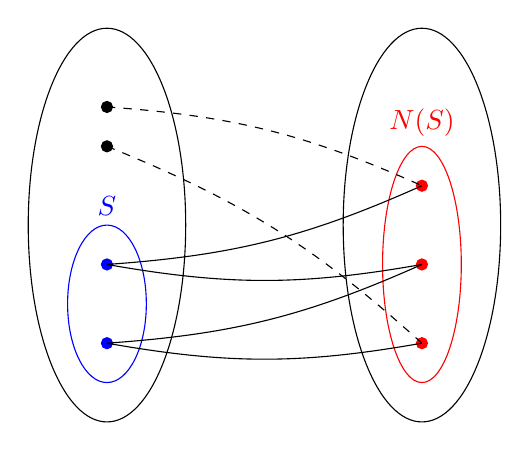
\begin{tikzpicture}
    \coordinate (L1) at (-2, -0.5);
    \coordinate (L2) at (-2, -1.5);

    \coordinate (LS1) at (-2, 1.5);
    \coordinate (LS2) at (-2, 1);

    \coordinate (R1) at (2, 0.5);
    \coordinate (R2) at (2, -0.5);
    \coordinate (R3) at (2, -1.5);

    \draw (-2, 0) ellipse (1cm and 2.5cm);
    \draw (2, 0) ellipse (1cm and 2.5cm);

    \begin{scope}[every path/.style = {color = blue}]
      \draw (-2, -1) ellipse (0.5cm and 1cm);
      \draw node[above] at (-2, 0) {\(S\)};
      \draw[fill = blue] (L1) circle (2pt);
      \draw[fill = blue] (L2) circle (2pt);
    \end{scope}

    \draw[fill = black] (LS1) circle (2pt);
    \draw[fill = black] (LS2) circle (2pt);

    \begin{scope}[every path/.style = {color = red}]
      \draw (2,-0.5) ellipse (0.5cm and 1.5cm);
      \draw node[above] at (2, 1) {\(N(S)\)};
      \draw[fill = red] (R1) circle (2pt);
      \draw[fill = red] (R2) circle (2pt);
      \draw[fill = red] (R3) circle (2pt);
    \end{scope}

    \draw (L1) edge[bend right = 10] (R1);
    \draw (L1) edge[bend right = 10] (R2);
    \draw (L2) edge[bend right = 10] (R2);
    \draw (L2) edge[bend right = 10] (R3);

    \draw[dashed] (LS1) edge[bend left = 10] (R1);
    \draw[dashed] (LS2) edge[bend left = 10] (R3);
  \end{tikzpicture}  
\end{figure}
\end{twocolumns}

  \question{Интегрирование некоторых иррациональных функций, метод тригонометрической подстановки.}

\begin{itemize}
\item Интегралы вида \(\int R(\sqrt{x^2 \pm 1}, x) \dd x\) решаются с помощью
замены \(x\) на гиперболическую функцию:

\begin{align*}
  \sinh u = \frac{e^u - e^{-u}}{2} \qquad
  \cosh u = \frac{e^u + e^{-u}}{2}
\end{align*}

Данные функции называются гиперболическим синусом и гиперболическим косинусом
соответственно.

\begin{lemma}
  Основное гиперболическое тождество

  \begin{align*}
    \cosh^2 u - \sinh^2 u = 1
  \end{align*}
\end{lemma}
\begin{proof}
  \begin{align*}
    \cosh^2 u - \sinh^2 u=
    \left(\frac{e^{u} + e^{-u}}{2}\right)^2
      - \left(\frac{e^{u} - e^{-u}}{2}\right)^2 =
    \frac{1}{4} \left(e^{2u} + 2 + e^{-2u} - e^{2u} + 2 - e^{-2u} \right) = 1
  \end{align*}
\end{proof}

\begin{remark}\label{hpr-rep}
  Заметим, что

  \begin{align*}
    \ln \abs{\sinh u + \cosh u}
    = \ln \abs{\frac{e^u - e^{-u}}{2} + \frac{e^u + e^{-u}}{2}}
    = \ln e^{u}
    = u
  \end{align*}
\end{remark}

\begin{example}
  Вычислим 'длинный' логарифм:

  \begin{align*}
    \int \frac{\dd x}{\sqrt{1 + x^2}} = 
    \begin{bmatrix}
      x = \sinh u \implies 1 + x^2 = \cosh^2 u \\
      \dd x = \dd (\sinh u) = \cosh u \dd u \\
      u = \ln \abs{
        \under{x}{\sinh u} + \under{\sqrt{1 + x^2}}{\cosh u}
      } \;\; (\ref{hpr-rep})
    \end{bmatrix} =
    \int \frac{\cosh u}{\cosh u} \dd u =
    u + C =
    \ln \abs{x + \sqrt{1 + x^2}} + C
  \end{align*}
\end{example}

\item Интегралы вида \(\int R(\sqrt{1 - x^2}, x) \dd x\) решаются с помощью
замены \(x\) на синус или косинус.

\item Интегралы вида \(\int R(\sqrt[k_{1}]{x}, \dots, \sqrt[k_{n}]{x}) \dd x\)
решаются с помощью замены \(t = \sqrt[K]{x}\), где \(K\) это НОК для
\(k_{1}, \dotsc, k_{n}\).

\item Интегралы вида \(\int R(\sqrt{ax + b}, x) \dd x\) решаются с помощью
замены \(t = \sqrt{ax + b}\). При этом \(x = \frac{t^2 - b}{a}\),
\(\dd x = \frac{2t}{a} \dd t\).
\end{itemize}

  \subsection{%
  Сравнение бесконечно малых. Теоремы об эквивалентных функциях.%
}

Пусть \(\infsmall_1(x)\) и \(\infsmall_2(x)\)~--- б.м. в точке \(a\), тогда

\begin{enumerate}
\item
  \(
    \lim_{x \to a} \frac{\infsmall_1(x)}{\infsmall_2(x)} = 0
    \implies \infsmall_1(x)
  \) более высокого порядка, чем \(\infsmall_2(x)\).

\item
  \(
    \lim_{x \to a} \frac{\infsmall_1(x)}{\infsmall_2(x)} \in \RR \setminus
    \set{0} \implies \infsmall_1(x)
  \) и \(\infsmall_2(x)\) одного порядка.

\item
  \(
    \lim_{x \to a} \frac{\infsmall_1(x)}{\infsmall_2(x)} = \infty
    \implies \infsmall_1(x)
  \) более низкого порядка, чем \(\infsmall_2(x)\).

\item
  \(
    \lim_{x \to a} \frac{\infsmall_1(x)}{\infsmall_2(x)^k} \in \RR \setminus
    \set{0} \implies \infsmall_1(x)
  \) имеет порядок \(k\) по отношению к \(\infsmall_2(x)\).
\end{enumerate}

Пусть \(\infbig_1(x)\) и \(\infbig_2(x)\)~--- б.б. в точке \(a\), тогда

\begin{enumerate}
\item
  \(
    \lim_{x \to a} \frac{\infbig_1(x)}{\infbig_2(x)} = 0
    \implies \infbig_1(x)
  \) более низкого порядка, чем \(\infbig_2(x)\).

\item
  \(
    \lim_{x \to a} \frac{\infbig_1(x)}{\infbig_2(x)} \in \RR \setminus
    \set{0} \implies \infbig_1(x)
  \) и \(\infbig_2(x)\) одного порядка.

\item
  \(
    \lim_{x \to a} \frac{\infbig_1(x)}{\infbig_2(x)} = \infty
    \implies \infbig_1(x)
  \) более высокого порядка, чем \(\infbig_2(x)\).

\item
  \(
    \lim_{x \to a} \frac{\infbig_1(x)}{\infbig_2(x)^k} \in \RR \setminus
    \set{0} \implies \infbig_1(x)
  \) имеет порядок \(k\) по отношению к \(\infbig_2(x)\).
\end{enumerate}

\begin{remark}
  \(\smallo(f(x))\)~--- обозначение б.м. более высокого порядка для функции
  \(f(x)\). Обычно это обозначение используют для сравнения с некоторым эталоном
  \(\Delta x\), например

  \begin{equation*}
    \infsmall(x) = \smallo(\Delta x)
    \iff
    \lim_{x \to a} \frac{\infsmall(x)}{\Delta x} = 0
  \end{equation*}
\end{remark}

\begin{remark}
  Таким образом, разрешение неопределенностей вида
  \(\display{\left[\frac{0}{0}\right]}\) и
  \(\display{\left[\frac{\infty}{\infty}\right]}\) это на самом деле сравнение
  бесконечно малых и бесконечно больших функций.
\end{remark}

\begin{definition}
  Если \(\lim_{x \to a} \frac{\infsmall_1(x)}{\infsmall_2(x)} = 1\), то
  \(\infsmall_1(x)\) и \(\infsmall_2(x)\) называются эквивалентными б.м.
  функциями.

  \begin{equation*}
    \lim_{x \to a} \frac{\infsmall_1(x)}{\infsmall_2(x)} = 1
    \iff
    \infsmall_1(x) \sim \infsmall_2(x)
  \end{equation*}
\end{definition}

\begin{remark}
  Геометрический смысл эквивалентных функций заключается в том, что в малой
  окрестности точки \(a\) графики функций сливаются. В качестве примера можно
  рассмотреть функции \(\sin x\) и \(x\) (\figref{01_08_01}).
\end{remark}

\galleryone{01_08_01}{Эквивалентные функции}

\begin{theorem}
  В произведении можно заменять эквивалентные функции друг на друга при
  условии, что они эквивалентны \textbf{в одной точке}.

  \begin{equation*}
    \alpha(x) \sim \gamma(x)
    \implies
    \lim_{x \to a} \frac{\infsmall(x)}{\beta(x)}
    = \lim_{x \to a} \frac{\gamma(x)}{\beta(x)}
  \end{equation*}
\end{theorem}

\begin{proof}
  Домножим на \(\gamma(x)\) и воспользуемся свойством произведения пределов.

  \begin{equation*}
    \lim_{x \to a} \frac{\alpha(x)}{\beta(x)} 
    = \lim_{x \to a} \frac{\alpha(x) \cdot \gamma(x)}{\beta(x) \cdot \gamma(x)}
    = \lim_{x \to a} \frac{\alpha(x)}{\gamma(x)} \cdot
      \lim_{x \to a} \frac{\gamma(x)}{\beta(x)}
  \end{equation*}

  По определению эквивалентных функций левый предел равен единице, значит

  \begin{equation*}
    \lim_{x \to a} \frac{\alpha(x)}{\beta(x)}
    = \lim_{x \to a} \frac{\gamma(x)}{\beta(x)}
  \end{equation*}
\end{proof}

\begin{theorem}
  Разность эквивалентных \textbf{в одной точке} б.м. функций это б.м. более
  высокого порядка, чем эти функции.

  \begin{equation*}
    \alpha(x) \sim \beta(x)
    \implies
    \alpha(x) - \beta(x) = \smallo(\alpha(x)) = \smallo(\beta(x))
  \end{equation*}
\end{theorem}

\begin{proof}
  Сравним \(\alpha(x) - \beta(x)\) по определению сравнения б.м. функций, для
  этого вычислим следующий предел

  \begin{equation*}
    \lim_{x \to a} \frac{\alpha(x) - \beta(x)}{\alpha(x)}
    = \lim_{x \to a} 1 - \frac{\beta(x)}{\alpha(x)}
    = 1 - \lim_{x \to a} \frac{\beta(x)}{\alpha(x)}
  \end{equation*}

  По определению эквивалентных функций правый предел равен единице, значит

  \begin{equation*}
    \lim_{x \to a} \frac{\alpha(x) - \beta(x)}{\alpha(x)}
    = 1 - 1
    = 0
  \end{equation*}

  Таким образом \(\alpha(x) - \beta(x)\) это б.м. более высокого порядка, чем
  \(\alpha(x)\). Для \(\beta(x)\) доказательство аналогично.
\end{proof}

\begin{theorem}
  Произведение двух б.м. \textbf{в одной точке} функций это б.м. более высокого
  порядка, чем эти функции.

  \begin{equation*}
    \alpha(x) \cdot \beta(x) = \smallo(\alpha(x)) = \smallo(\beta(x))
  \end{equation*}
\end{theorem}

\begin{proof}  
  Сравним \(\alpha(x) \cdot \beta(x)\) по определению сравнения б.м. функций,
  для этого вычислим следующий предел

  \begin{equation*}
    \lim_{x \to a} \frac{\alpha(x) \cdot \beta(x)}{\alpha(x)}
    = \lim_{x \to a} \beta(x)
  \end{equation*}

  По определению б.м. функции этот предел равен нулю. Таким образом \(\alpha(x)
  \cdot \beta(x)\) это б.м. более высокого порядка, чем \(\alpha(x)\). Для
  \(\beta(x)\) доказательство аналогично.
\end{proof}

  \question{Геометрический смысл определенного интеграла. Оценка определенного интеграла. Теорема о среднем.}


  \question{Структура образа самосопряженного оператора. Проектор. Спектральное разложение оператора.}

\begin{theorem}\label{sconj-lo-img}
  Образ самосопряженного оператора \(\opA \colon V^{n} \to V^{n}\) имеет вид

  \begin{align*}
    \Img \opA = \left\{
      \sum_{i = 1}^{n}
      \lambda_{i} (x, \basis_{i}) \basis_{i}
      \mid x \in V^{n}
    \right\}
  \end{align*}

  где \(\Basis = \{ \basis_{i} \}_{i = 1}^{n}\) это ортонормированный базис,
  \(\lambda_{i}\)~--- собственные числа оператора \(\opA\).
\end{theorem}
\begin{proof}
  \begin{align*}
    \opA x = y =
    \\
      y_{1} \basis_{1}
        + \dotsc + y_{n} \basis_{n} =
    \\
      (y, \basis_{1}) \basis_{1}
        + \dotsc + (y, \basis_{n}) \basis_{n} =
    \\
      (\opA x, \basis_{1}) \basis_{1}
        + \dotsc + (\opA x, \basis_{n}) \basis_{n} =
    \\
      (x, \opA \basis_{1}) \basis_{1}
        + \dotsc + (x, \opA \basis_{n}) \basis_{n} =
    \\
      (x, \lambda_{1} \basis_{1}) \basis_{1}
        + \dotsc + (x, \lambda_{n} \basis_{n}) \basis_{n} =
    \\
      \lambda_{1} (x, \basis_{1}) \basis_{1}
        + \dotsc + \lambda_{n} (x,\basis_{n}) \basis_{n} =
    \\
    \sum_{i = 1}^{n} \lambda_{i} (x, \basis_{i}) \basis_{i}
  \end{align*}
\end{proof}

\begin{remark}
  \((x, \basis_{i})\) это проекция вектора \(x\) на собственный вектор.

  Таким образом \(y\) получается следующим образом: \(x\) проецируется на 
  \(\basis_{1}, \dotsc, \basis_{n}\), после чего проекции 'растягиваются' в
  \(\lambda_{1}, \dotsc, \lambda_{n}\) раз и суммируются.
\end{remark}

\begin{definition}\label{lo-proj}
  Оператор вида

  \begin{align*}
    P_{i}(x) = (x, \basis_{i}) \basis_{i}
  \end{align*}

  называется проектором на одномерное пространство, порожденное собственным
  вектором.
\end{definition}

\begin{remark}
  Проектор является самосопряженным оператором.
\end{remark}

\begin{definition}
  Спектральным разложением оператора называется представление его в виде
  линейной комбинации проекторов

  \begin{align*}
    \opA = \sum_{i = 1}^{n} \lambda_{i} P_{i}
  \end{align*}

  Корректность такого представления следует из \ref{sconj-lo-img} и
  \ref{lo-proj}.
\end{definition}
  \question{Свойства решений ЛОДУ\(_2\): линейная независимость решений, определитель Вронского. Теоремы 1,2.}

Рассмотрим множество \(\Omega\) непрерывных функций с непрерывными производными
2ого порядка. Определим линейный дифференциальный оператор
\(\Linear{y} = y'' + py' + qy \to f(x)\).

\begin{definition}
  Будем называть функции \(y_{1}, \dotsc, y_{n}\) линейно-независимыми на
  отрезке \([a; b]\), если

  \begin{align*}
    \sum_{i = 1}^{n} c_{i} y_{i} = 0 \implies \forall c_{i} = 0
  \end{align*}
\end{definition}

\begin{definition}
  Определитель Вронского (вронскиан) \(\Wrn\) это определитель, составленный из
  \(n\) функций и всех их производных вплоть до \((n - 1)\)-ого порядка. Он
  имеет вид:

  \begin{align*}
    \Wrn = \begin{vmatrix}
      y_{1}  & \dotsc  & y_{n} \\
      \vdots & \ddots & \vdots \\
      y^{(n - 1)}_{1}  & \dotsc  & y^{(n - 1)}_{n}
    \end{vmatrix}
  \end{align*}
\end{definition}

\begin{lemma}\label{wrn-prop-1}
  Если два решения ЛОДУ\(_2\) линейно-зависимы на \([a; b]\), то их
  вронскиан на \([a; b]\) равен нулю.

  \begin{align*}
    \begin{rcases}
      \Linear{y_{1}} = 0 \\
      \Linear{y_{2}} = 0 \\
      y_{1} = \lambda y_{2}
    \end{rcases} \implies \Wrn = 0
  \end{align*}
\end{lemma}
\begin{proof}
  \begin{align*}
    \Wrn = \begin{vmatrix}
      y_{1} & y_{2} \\
      y'_{1} & y'_{2} \\
    \end{vmatrix} = \begin{vmatrix}
      \lambda y_{2} & y_{2} \\
      \lambda y'_{2} & y'_{2} \\
    \end{vmatrix} = \lambda \begin{vmatrix}
      y_{2} & y_{2} \\
      y'_{2} & y'_{2} \\
    \end{vmatrix} = 0
  \end{align*}
\end{proof}

\begin{lemma}\label{wrn-prop-2}
  Если два решения ЛОДУ\(_2\) линейно-независимы на \([a; b]\), то их
  вронскиан на \([a; b]\) не равен нулю.

  \begin{align*}
    \begin{rcases}
      \Linear{y_{1}} = 0 \\
      \Linear{y_{2}} = 0 \\
      y_{1} \neq \lambda y_{2}
    \end{rcases} \implies \Wrn \neq 0
  \end{align*}
\end{lemma}
\begin{proof}
  От противного
  \begin{align*}
    \lets \Wrn = 0 = \begin{vmatrix}
      y_{1} & y_{2} \\
      y'_{1} & y'_{2} \\
    \end{vmatrix} = y_{1} y'_{2} - y'_{1} y_{2} \mid \colon y_{1}^{2} \neq 0 \\
    \frac{y_{1} y'_{2} - y'_{1} y_{2}}{y_{1}^{2}} = 0 \\
    \left(\frac{y_{2}}{y_{1}}\right)' = 0 \\
    \frac{y_{2}}{y_{1}} = const \\
    y_{1} = \lambda y_{2}
  \end{align*}
  Получили противоречие.
\end{proof}

\begin{theorem}
  Линейная зависимость/независимость функций определяется равенством их
  вронскиана нулю.
\end{theorem}
\begin{proof}
  Следствие из \ref{wrn-prop-1} и \ref{wrn-prop-2}.
\end{proof}

\begin{remark}
  Для проверки набора функций на линейную зависимость/независимость лучше
  использовать именно вронскиан, а не непосредственное определение линейной
  зависимости функций на отрезке.
\end{remark}

\begin{theorem}\label{wrn-prop-3}
  Рассмотрим функции на отрезке \([a; b]\). Если на этом отрезке найдется точка,
  в которой вронскиан равен нулю, вронскиан будет равен нулю на всем отрезке.
  Дуально, если найдется точка, в которой вронскиан не равен нулю, то он будет
  не равен нулю на всем отрезке.

  \begin{align*}
    \exists x_{0} \in [a; b] \mid W(x_{0}) = W_{0} \neq 0
      \implies \forall x \in [a, b] \colon W(x) \neq 0 \\
    \exists x_{0} \in [a; b] \mid W(x_{0}) = W_{0} = 0
      \implies \forall x \in [a, b] \colon W(x) = 0 \\
  \end{align*}
\end{theorem}
\begin{proof}
  Пусть \(y_{1}\) и \(y_{2}\) это решения ДУ, тогда

  \begin{align*}
    \begin{cases}
      y_{2}'' + p y_{2}' + q y_{2} = 0 \mid \cdot \; y_{1} \\
      y_{1}'' + p y_{1}' + q y_{1} = 0 \mid \cdot \; y_{2}
    \end{cases} - \\
    (y_{1} y_{2}'' - y_{2} y_{1}'') + p (y_{1} y_{2}' - y_{1}' y_{2}) = 0
  \end{align*}

  Заметим, что выражение в левой скобке это \(\Wrn'\), а во правой~--- \(\Wrn\):

  \begin{align*}
    \Wrn = y_{1} y_{2}' - y_{1}' y_{2} \\
    \Wrn'
    = (y_{1} y_{2}' - y_{1}' y_{2})'
    = y_{1}' y_{2}' + y_{1} y_{2}'' - y_{1}'' y_{2} - y_{1}' y_{2}'
    = y_{1} y_{2}'' - y_{1}'' y_{2}
  \end{align*}

  Подставим это в полученное ранее уравнение:

  \begin{align*}
    (y_{1} y_{2}'' - y_{2} y_{1}'') + p (y_{1} y_{2}' - y_{1}' y_{2}) = 0 \\
    \Wrn' + p \Wrn = 0 \\
    \Wrn = c_{1} e^{-\int p \dd x} \\
    \Wrn(x_{0})
    = c_{1} e^{-\int_{x_{0}}^{x_{0}} p \dd x}
    = c_{1}
    = \Wrn_{0}
    \\
    \Wrn(x)
    = c_{1} e^{-\int_{x_{0}}^{x} p \dd x}
    = \Wrn_{0} e^{-\int_{x_{0}}^{x} p \dd x}
  \end{align*}

  Таким образом, если \(\Wrn_{0} = 0\), то \(\Wrn(x) = 0\) на всем отрезке
  \([a; b]\). Дуально, если \(\Wrn_{0} \neq 0\), то т.к. второй множитель всегда
  больше нуля, то \(\Wrn(x) \neq 0\).
\end{proof}

\begin{remark}
  Таким образом, чтобы узнать равен ли вронскиан нулю на отрезке, достаточно
  узнать его значение в одной произвольной точке этого отрезка.
\end{remark}

  \question{Деревья.}

\begin{definition}
  Дерево это связный ацикличный граф.
\end{definition}

\begin{definition}
  Лес это ацикличный граф, т.е. объединение непересекающихся деревьев.
\end{definition}

\begin{definition}
  Укорененное дерево это дерево, в котором одна из вершин обозначена корнем.
\end{definition}

\begin{definition}
  Предком вершины называется следующая вершина на кратчайшем пути к корню.
\end{definition}

\begin{definition}
  Если \(u\)~--- предок \(v\), то \(v\) называется ребенком \(u\).
\end{definition}

\begin{definition}
  Если у двух вершин один и тот же родитель, то они называются братьями.
\end{definition}

\begin{definition}
  Лист это вершина, у которой нет детей.
\end{definition}

\begin{definition}
  Вершины, не являющиеся листьями, называются внутренними.
\end{definition}

\begin{definition}
  Дерево называется \(k\)-арным, если все его вершины имеют не более \(k\)
  детей. Если \(k = 2\), то такое дерево называют бинарным.
\end{definition}

\begin{definition}
  Веткой вершины в дереве называется некоторый индуцированный подграф такой, что
  данная вершина является в нем корнем.
\end{definition}

\begin{definition}
  Вес ветки это сумма весов всех входящих в него ребер. Если дерево
  невзвешенное, то считаем вес каждого ребра равным единице.
\end{definition}

\begin{definition}
  Весом вершины называется максимальный из весов веток этой вершины.
\end{definition}

\begin{definition}
  Центроид дерева это множество вершин с минимальным весов.
\end{definition}

\begin{lemma}
  Центроид дерева содержит либо одну, либо две вершины.
\end{lemma}
\begin{proof}
  Рассмотрим невзвешенное дерево. На каждом шаге будем убирать все листья из
  текущего дерева, при этом степени оставшихся вершин будут уменьшаться на
  единицу. Будем так повторять, пока существует вершина со степенью более
  единицы.
  
  В итоге останется либо одна вершина со степенью ноль, либо две вершины со
  степенью один. Значит в исходном графе именно у этой вершины (или у этих двух
  вершин) была наименьшая степень.
\end{proof}

\begin{definition}
  Дерево называется помеченным, если каждой из его вершин соответствует
  уникальная метка от \(1\) до \(n\).
\end{definition}

\begin{definition}
  Код Прюфера эт уникальная последовательность меток от \(1\) до \(n\) длины
  \(n - 2\), которая соответствует уникальному помеченному дереву на \(n\)
  вершинах.
\end{definition}

\begin{lemma}
  Всего существует \(n^{n - 2}\) помеченных деревьев на \(n\) вершинах.
\end{lemma}
\begin{proof}
  Между деревьями на \(n\) вершинах и кодами Прюфера длина \(n -2\) действует
  биекция. Существует \(n^{n - 2}\) кодов Прюфера длины \(n - 2\).
\end{proof}

Кодирование
[\href{https://www.youtube.com/watch?v=Caqn-Vx4PoY}{визуализация}]:
\begin{enumerate}
  \item Выбираем лист с наименьшей меткой.
  \item Добавляем в ответ его родителя, после чего удаляем этот лист.
  \item Повторяем шаги \(1-2\) \(n - 2\) раза.
\end{enumerate}

Декодирование
[\href{https://www.youtube.com/watch?v=7s44l7gWEVk}{визуализация}]:
\begin{enumerate}
  \item Выписываем в строку все метки от \(1\) до \(n\).
  \item Среди выписанных меток ищем первую, которой нет в коде Прюфера.
  \item Добавляем в граф ребро между найденной меткой и первой меткой в коде
  Прюфера.
  \item Удаляем найденную метку из последовательности меток, а также удаляем
  первый элемент в коде Прюфера
  \item Повторяем шаги \(2-4\) пока не закончится код Прюфера.
  \item В последовательности останется \(2\) метки, добавляем ребро между ними.
\end{enumerate}

\begin{remark}
  Кодировать и декодировать код Прюфера можно за \(O(n)\). Алгоритм описан
  \href{https://www.scirp.org/pdf/JSEA20090200006_93737200.pdf}{здесь}.
\end{remark}
  \question{Квадратичная форма: определения, приведение к каноническому виду.}

\begin{definition}
  Числовая функция одного аргумента \(\Quad(u) \mid u \in V^{n}\), которая
  порождается билинейной формой \(\BiLinear(u, v)\) при \(u = v\) называется
  квадратичной формой.

  \begin{lequation}{quad-form-def}
    \Quad(u) = \BiLinear(u, u)
  \end{lequation}
\end{definition}

\begin{remark}
  Если квадратичная форма порождена симметричной билинейной формой, то эта
  билинейная форма называется полярной для квадратичной.
\end{remark}

\begin{definition}
  Каноническим видом квадратичной формы \(\Quad^{d}(u)\) является сумма
  квадратов с некоторыми коэффициентами.

  \begin{lequation}{quad-can}
    \Quad^{d}(u) = \lambda_{1} u_{1}^{2} + \dotsc + \lambda_{n} u_{n}^{2}
  \end{lequation}

  Причем \(\lambda_{i}\) называются каноническими коэффициентами.
\end{definition}

\begin{definition}
  Если в каноническом виде все коэффициенты \(\lambda_{i}\) равны \(\pm 1\) или
  \(0\), то такой вид называется нормальным.
\end{definition}

\begin{definition}
  Базис, в котором квадратичная форма является канонической, называется
  каноническим базисом.
\end{definition}

\begin{remark}
  Канонический базис не единственный.
\end{remark}

\begin{remark}
  Пусть квадратичная форма задана в виде

  \begin{lequation}{quad-mtx-1}
    \Quad(u)
    = a_{1,1} u_{1}^2 + \dotsc + a_{n,n} u_{n}^2
    + 2 a_{1,2} u_{1} u_{2} + \dotsc + 2 a_{1,n} u_{1} u_{n}
    + \dotsc
    + 2 a_{n,1} u_{n} u_{1} + \dotsc + 2 a_{n,n - 1} u_{n} u_{n - 1}
  \end{lequation}

  тогда её матрица будет иметь вид

  \begin{lequation}{quad-mtx-1}
    \begin{pmatrix}
      a_{1,1} & \dots  & a_{1,n} \\
      \vdots  & \ddots & \vdots \\
      a_{n,1} & \dots  & a_{n,n} \\
    \end{pmatrix}
  \end{lequation}
\end{remark}

\begin{theorem}
  Всякую квадратичную форму \(\Quad(u)\) можно привести к каноническому
  виду невырожденным преобразованием.
\end{theorem}
\begin{proof}
  не потребуется на экзамене)
\end{proof}

\underline{Метод Лагранжа}:

Один из способов приведения квадратичной формы к каноническому виду.

Рассмотрим его на примере \(
  \Quad(x)
  = x_{1}^2 + 9 x_{2}^2 + x_{3}^2
  + 6 x_{1} x_{2} + 2 x_{1} x_{3} + 2 x_{2} x_{3}
\)

Метод заключается в последовательном выделении полных квадратов:

\begin{lequation}{quad-L-ex-1}
  x_{1}^2 + 9 x_{2}^2 + x_{3}^2 +
  6 x_{1} x_{2} + 2 x_{1} x_{3} + 2 x_{2} x_{3}
  \\
  x_{1}^2 + 2 x_{1} (3 x_{2} + x_{3}) + 9 x_{2}^2 + x_{3}^2 + 2 x_{2} x_{3}
  \\
  \Big( x_{1}^2 + 2 x_{1} (3 x_{2} + x_{3}) + (3 x_{2} + x_{3})^2 \Big)
  - (3 x_{2} + x_{3})^2 + 9 x_{2}^2 + x_{3}^2 + 2 x_{2} x_{3}
  \\
  (x_{1} + 3 x_{2} + x_{3})^2
  - 9 x_{2}^2 - 6 x_{2} x_{3} - x_{3}^2
  + 9 x_{2}^2 + x_{3}^2 + 2 x_{2} x_{3} 
  \\
  (x_{1} + 3 x_{2} + x_{3})^2 - 4 x_{2} x_{3} 
\end{lequation}

Далее делаем замену

\begin{lequation}{quad-L-ex-2}
  \begin{cases}
    y_{1} = x_{1} + 3 x_{2} + x_{3} \\
    y_{2} = \frac{1}{2} (x_{2} + x_{3}) \\
    y_{3} = \frac{1}{2} (x_{2} - x_{3})
  \end{cases}
\end{lequation}

Замены \(y_{2}\) и \(y_{3}\) именно такие, потому что остался моном
\(- 4 x_{2} x_{3}\), из которого мы не можем выделить полный квадрат.

\begin{lequation}{quad-L-ex-3}
  \begin{cases}
    y_{2} = \frac{1}{2} (x_{2} + x_{3}) \\
    y_{3} = \frac{1}{2} (x_{2} - x_{3})
  \end{cases} \implies
  \begin{cases}
    x_{2} = y_{2} + y_{3} \\
    x_{3} = y_{2} - y_{3}  
  \end{cases} \\
  (x_{1} + 3 x_{2} + x_{3})^2 - 4 x_{2} x_{3}  \\
  y_{1}^2 - 4 (y_{2} + y_{3}) (y_{2} - y_{3}) \\
  y_{1}^2 - 4 (y_{2}^2 - y_{3}^2) \\
  y_{1}^2 - 4 y_{2}^2 + 4 y_{3}^2 \\
\end{lequation}

Таким образом, получен канонический вид квадратичной формы 
\(\Quad^{d}(y) = y_{1}^2 - 4 y_{2}^2 + 4 y_{3}^2\).

Матрицу полученного преобразования можно получить из уравнения \(x = P y\), для
этого обратимся к сделанной замене и найдем обратную матрицу:

\begin{lequation}{quad-L-ex-4}
  y = \begin{pmatrix}
    1 & 3            & 1             \\
    0 & \sfrac{1}{2} & \sfrac{1}{2}  \\
    0 & \sfrac{1}{2} & -\sfrac{1}{2}
  \end{pmatrix}
  x
  \\
  x = \begin{pmatrix}
    1 & 3            & 1             \\
    0 & \sfrac{1}{2} & \sfrac{1}{2}  \\
    0 & \sfrac{1}{2} & -\sfrac{1}{2}
  \end{pmatrix}^{-1}
  y
  \\
  P = \begin{pmatrix}
    1 & -4 & -2 \\
    0 &  1 &  1 \\
    0 &  1 & -1
  \end{pmatrix}
\end{lequation}

Пусть \(K\) это матрица квадратичной формы \(\Quad(x)\) в исходном базисе, а
\(K^{d}\)~--- в диагональном. Тогда проверить корректность найденной матрицы
преобразования можно следующим образом:

\begin{lequation}{quad-L-ex-5}
  K^{d} = P^{T} K P = 
  \begin{pmatrix}
    1  & 0 &  0 \\
    -4 & 1 &  1 \\
    -2 & 1 & -1
  \end{pmatrix}
  \begin{pmatrix}
    1 & 3 & 1 \\
    3 & 9 & 1 \\
    1 & 1 & 1
  \end{pmatrix}
  \begin{pmatrix}
    1 & -4 & -2 \\
    0 &  1 &  1 \\
    0 &  1 & -1
  \end{pmatrix}
  =
  \begin{pmatrix}
    1 &  0 & 0 \\
    0 & -4 & 0 \\
    0 &  0 & 4
  \end{pmatrix}
\end{lequation}

\underline{Ортоногальное преобразование}:

Метод, позволяющий привести квадратичную форму к каноническому виду с
помощью ортогонального преобразования.

Рассмотрим его на примере \(\Quad(x) = x_{1}^2 + x_{2}^2 - 4 x_{1} x_{2}\).

Сначала составим матрицу квадратичной формы, после чего найдем её собственные
числа и собственные векторы:

\begin{lequation}{quad-ort-ex-1}
  \begin{pmatrix}
     1 & -2 \\
    -2 & 1
  \end{pmatrix}
  \implies
  \begin{cases}
    \lambda_{1} = -1 \\
    \lambda_{2} = 3
  \end{cases}
  \implies
  \begin{cases}
    \basis_{1} = \begin{pmatrix} 1 \\ 1 \end{pmatrix} \\
    \basis_{2} = \begin{pmatrix} 1 \\ -1 \end{pmatrix}
  \end{cases}
\end{lequation}

Найденные собственные числа будут коэффициентами при квадратах в диагональном
виде квадратичной формы \(\Quad^{d}(y) = -y_{1}^2 + 3 y_{2}^2\).

Далее нормируем полученные собственные векторы и используем их как столбцы
матрицы ортогонального преобразования \(P\):

\begin{lequation}{quad-ort-ex-2}
  \begin{cases}
    \basis_{1} = \begin{pmatrix} 1 \\ 1 \end{pmatrix} \\
    \basis_{2} = \begin{pmatrix} 1 \\ -1 \end{pmatrix}
  \end{cases}
  \implies
  \begin{cases}
    \widehat{\basis_{1}} = \begin{pmatrix}
      \sfrac{1}{\sqrt{2}} \\
      \sfrac{1}{\sqrt{2}}
    \end{pmatrix}
    \\
    \widehat{\basis_{2}} = \begin{pmatrix}
      \sfrac{1}{\sqrt{2}} \\
      \sfrac{-1}{\sqrt{2}}
    \end{pmatrix}
  \end{cases}
  \implies
  P = \begin{pmatrix}
    \sfrac{1}{\sqrt{2}} & \sfrac{1}{\sqrt{2}} \\
    \sfrac{1}{\sqrt{2}} & \sfrac{-1}{\sqrt{2}} \\
  \end{pmatrix}
\end{lequation}

\begin{remark}
  Ранг матрицы квадратичной формы это инвариант относительно любого
  невырожденного преобразования.
\end{remark}
  \subsection{%
  Лекция \texttt{23.12.05}.%
}

\subheader{Характеристические функции}

Пусть \(\xi + i \eta\)~--- комплексная случайная величина, причем \(\xi\) и
\(\eta\) это обычные случайные величины с конечным первым моментом.

\begin{definition}
  Математическое ожидание комплекснозначной случайной величины определим как

  \begin{equation*}
    \expected{\xi + i \eta} = \expected{\xi} + i \expected{\eta}
  \end{equation*}
\end{definition}

\begin{definition}
  Характеристической функцией случайной величины \(\xi\) называется функция

  \begin{equation*}
    \phi_{\xi} (t) = \expected{e^{i \xi t}}
    \qquad
    t \in \RR
  \end{equation*}
\end{definition}

\begin{lemma}
  Характеристическая функция существует для любой случайной величины \(\xi\),
  причем \(\abs{\phi_{\xi} (t)} \le 1\).  
\end{lemma}

\begin{proof}
  Заметим, что

  \begin{equation*} \label{eq:char-func-lim-1} \tag{1}
    \variance{\xi} = \expected{\xi^2} - \prh{\expected{\xi}}^2 \ge 0
    \implies
    \prh{\expected{\xi}}^2 \le \expected{\xi^2}
  \end{equation*}

  Оценим модуль характеристической функции.

  \begin{equation*} \label{eq:char-func-lim-2} \tag{2}
    \begin{aligned}
      \abs{\phi_{\xi} (t)}^2
      & = \abs{\expected{e^{i \xi t}}}^2
    \\
      & = \abs{\expected{\cos (\xi t) + i \sin (\xi t)}}^2
    \\
      & = \abs{\expected{\cos (\xi t)} + i \expected{\sin (\xi t)}}^2
    \\
      & = \abs{\expected{\cos (\xi t)}}^2 + \abs{\expected{\sin (\xi t)}}^2
    \end{aligned}
  \end{equation*}

  Применим к полученному в \eqref{eq:char-func-lim-2} неравенство из
  \eqref{eq:char-func-lim-1}, получим

  \begin{equation*}
    \abs{\phi_{\xi} (t)}^2
    \le \expected{\cos^2 (\xi t)} + \expected{\sin^2 (\xi t)}
    = \expected{\cos^2 (\xi t) + \sin^2 (\xi t)}
    = \expected{1}
    = 1
  \end{equation*}
\end{proof}

\begin{lemma} \label{lem:char-func-lin-transform}
  Пусть \(\phi_{\xi} (t)\) это характеристическая функция случайной величины
  \(\xi\). Тогда характеристическая функция случайной величины \(\eta = a + b
  \xi\) будет иметь вид

  \begin{equation*}
    \phi_{a + b \xi} (t) = e^{i t a} \cdot \phi_{\xi} (b t)
  \end{equation*}
\end{lemma}

\begin{proof}
  \begin{equation*}
    \phi_{a + b \xi} (t)
    = \expected{e^{i (a + b \xi) t}}
    = \expected{e^{i a t} \cdot e^{i b \xi t}}
    = e^{i a t} \expected{e^{i (b t) \xi}}
    = e^{i t a} \cdot \phi_{\xi} (b t)
  \end{equation*}  
\end{proof}

\begin{lemma} \label{lem:char-func-sum-ind}
  Характеристическая функция суммы независимых случайных величин равна
  произведению их характеристических функций.
\end{lemma}

\begin{proof}
  Пусть случайные величины \(\xi\) и \(\eta\) независимы, тогда

  \begin{equation*}
    \phi_{\xi + \eta} (t)
    = \expected{e^{i (\xi + \eta) t}}
    = \expected{e^{i \xi t} \cdot e^{i \eta t}}
    = \expected{e^{i \xi t}} \cdot \expected{e^{i \eta t}}
    = \phi_{\xi} (t) \phi_{\eta} (t)
  \end{equation*}
\end{proof}

\begin{lemma} \label{lem:char-func-series}
  Пусть \(\expected{\xi^k} < \infty\). Тогда

  \begin{equation*}
    \phi_{\xi} (t)
    = 1 + i t \cdot \expected{\xi} - \frac{t^2}{2} \expected{\xi^2}
      + \dotsc + \frac{i^k \expected{\xi^k}}{k!} t^k
      + \smallo \prh{\abs{t}^k}
  \end{equation*}
\end{lemma}

\begin{proof}
  Разложим экспоненту в ряд Маклорена и воспользуемся свойствами математического
  ожидания.

  \begin{equation*}
    \phi_{\xi} (t)
    = \expected{e^{i \xi t}}
    = \expected{
      1 + i \xi t + \frac{(i \xi t)^2}{2!}
      + \dotsc + \frac{(i \xi t)^k}{k!}
      + \smallo \prh{\abs{t}^k}
    }
    = 1 + i t \cdot \expected{\xi} - \frac{t^2}{2} \expected{\xi^2}
      + \dotsc + \frac{i^k \expected{\xi^k}}{k!} t^k
      + \smallo \prh{\abs{t}^k}
  \end{equation*}
\end{proof}

\begin{lemma}
  Пусть \(\expected{\xi^k} < \infty\). Тогда характеристическая функция
  непрерывно дифференцируема \(k\) раз, причем

  \begin{equation*}
    \phi_{\xi}^{(k)} (0) = i^k \expected{\xi^k}
  \end{equation*}
\end{lemma}

\begin{proof}
  Это следует из существования \(k\)-ого члена разложения характеристической
  функции в ряд Маклорена и равенства коэффициентов разложения:

  \begin{equation*}
    \frac{\phi_{\xi}^{(k)} (0)}{k!}
    = \frac{i^k \expected{\xi^k}}{k!}
    \implies
    \phi_{\xi}^{(k)} (0) = i^k \expected{\xi^k}
  \end{equation*}
\end{proof}

\begin{remark}
  Существует взаимнооднозначное соответствие между распределениями и
  характеристическими функциями. По характеристической функции можно
  восстановить распределение. В частности, если \(\xi\) абсолютно непрерывная
  случайная величина, то плотность можно найти по формуле

  \begin{equation*}
    f_{\xi} (x) = \frac{1}{\sqrt{2 \pi}} \int_{-\infty}^{\infty}
      e^{-i t \xi} \phi_{\xi} (t) \dd t
  \end{equation*}

  Это обратное преобразование Фурье.
\end{remark}

\begin{theorem}[О непрерывном соответствии] \label{thr:cont-match}
  Последовательность случайных величин \(\xi_n\) слабо сходится к случайной
  величине \(\xi\) тогда и только тогда, когда соответствующая
  последовательность характеристических функций поточечно сходится к
  характеристической функции случайной величины \(\xi\).

  \begin{equation*}
    \xi_n \rightrightarrows \xi
    \iff
    \phi_{\xi_n} (t) \to \phi_{\xi} (t)
    \qquad
    \forall t \in \RR
  \end{equation*}
\end{theorem}

\subheader{Характеристические функции стандартных распределений}

\subsubheader{I.}{Распределение Бернулли}

Пусть \(\xi \in B_p\), тогда

\begin{equation*}
  \phi_{\xi} (t)
  = \expected{e^{i \xi t}}
  = (1 - p) \expected{e^{i t \cdot 0}}
    + p \expected{e^{i t \cdot 1}}
  = 1 - p + p e^{i t}
\end{equation*}

\subsubheader{II.}{Биномиальное распределение}

Пусть \(\xi \in B_{n, p}\). Напомним, что

\begin{equation*}
  \prob{\xi = k} = \comb{n}{k} p^k q^{n - k}
  \qquad
  k = 0, 1, \dotsc, n
\end{equation*}

Тогда воспользуемся \ref{lem:char-func-sum-ind} и получим

\begin{equation*}
  \begin{aligned}
    \xi = \xi_1 + \dotsc + \xi_n
    \qquad
    \xi_i \in B_p
  \\
    \phi_{\xi} (t)
    = \prh{\phi_{\xi_1} (t)}^n
    = \prh{1 - p + p e^{i t}}^n
  \end{aligned}
\end{equation*}

\subsubheader{III.}{Распределение Пуассона}

Пусть \(\xi \in \Pi_{\lambda}\). Напомним, что

\begin{equation*}
  \prob{\xi = k} = \frac{\lambda^k}{k!} e^{-\lambda}
  \qquad
  k = 0, 1, \dotsc
\end{equation*}

Тогда получим

\begin{equation*}
  \phi_{\xi} (t)
  = \expected{e^{i \xi t}}
  = \sum_{k = 0}^{\infty} e^{i t k} \frac{\lambda^k}{k!} e^{-\lambda}
  = e^{-\lambda} \sum_{k = 0}^{\infty} \frac{\prh{\lambda e^{i t}}^k}{k!}
  = e^{-\lambda} \cdot e^{\lambda e^{i t}}
  = \exp \prh{\lambda \prh{e^{i t} - 1}}
\end{equation*}

\begin{lemma}
  Распределение Пуассона устойчиво относительно суммирования.
\end{lemma}

\begin{proof}
  Пусть даны независимые случайные величины \(\xi \in \Pi_{\lambda}\) и \(\eta
  \in \Pi_{\mu}\). Тогда по \ref{lem:char-func-sum-ind}

  \begin{equation*}
    \phi_{\xi + \eta} (t)
    = \phi_{\xi} (t) \phi_{\eta} (t)
    = \exp \prh{\lambda \prh{e^{i t} - 1}}
      \exp \prh{\mu \prh{e^{i t} - 1}}
    = \exp \prh{(\lambda + \mu) \prh{e^{i t} - 1}}
  \end{equation*}

  Получили характеристическую функцию распределения \(\Pi_{\xi + \eta}\).
\end{proof}

\subsubheader{IV.}{Показательное распределение}

Пусть \(\xi \in E_{\alpha}\). Напомним, что

\begin{equation*}
  f(x) = \begin{cases}
    0, & x < 0 \\
    \alpha e^{-\alpha x}, & x \ge 0
  \end{cases}
\end{equation*}

Тогда получим

\begin{equation*}
  \phi_{\xi} (t)
  = \expected{e^{i \xi t}}
  = \int_0^{+\infty} e^{i x t} \alpha e^{-\alpha x} \dd x
  = \alpha \int_0^{+\infty} e^{(i t - \alpha) x} \dd x
  = \frac{\alpha}{i t - \alpha} e^{(i t - \alpha) x} \Big\vert_0^{+\infty}
  = \frac{\alpha}{i t - \alpha} (0 - 1)
  = \frac{\alpha}{\alpha - i t}
\end{equation*}

\subsubheader{V.}{Стандартное нормальное распределение}

Пусть \(\xi \in N(0; 1)\). Напомним, что

\begin{equation*}
  f_{\xi} (x) = \frac{1}{\sqrt{2 \pi}} \exp \prh{-\frac{x^2}{2}}
  \qquad
  x \in \RR
\end{equation*}

Тогда получим

\begin{equation*}
  \begin{aligned}
    \phi_{\xi} (t)
    & = \expected{e^{i \xi t}}
  \\
    & = \int_{-\infty}^{\infty} e^{i t x}
      \frac{1}{\sqrt{2 \pi}} \exp \prh{-\frac{x^2}{2}} \dd x
  \\
    & = \frac{1}{\sqrt{2 \pi}} \int_{-\infty}^{\infty}
      \exp \prh{-\frac{1}{2} (x^2 - 2 i t x)} \dd x
  \\
    & = \frac{1}{\sqrt{2 \pi}} \int_{-\infty}^{\infty}
      \exp \prh{-\frac{1}{2} (x^2 - 2 i t x - t^2)}
      \exp \prh{-\frac{t^2}{2}} \dd x
  \\
    & = \frac{1}{\sqrt{2 \pi}} \exp \prh{-\frac{t^2}{2}}
      \under{
        \int_{-\infty}^{\infty} \exp \prh{-\frac{1}{2} (x - i t)^2}
        \dd (x - i t)
      }{\text{Интеграл Пуассона}}
  \\
    & = \frac{1}{\sqrt{2 \pi}} \exp \prh{-\frac{t^2}{2}} \sqrt{2 \pi}
  \\
    & = \exp \prh{-\frac{t^2}{2}}
  \end{aligned}
\end{equation*}
  
\subsubheader{VI.}{Нормальное распределение}

Пусть \(\xi \in N(a; \sigma^2)\). Нормируем ее и обозначим \(\eta = \frac{\xi -
a}{\sigma} \in N(0; 1)\). Характеристическая функция для нее уже найдена ранее:

\begin{equation*}
  \phi_{\eta} (t) = \exp \prh{-\frac{t^2}{2}}
\end{equation*}

Т.к. \(\xi = a + \eta \sigma\), то по \ref{lem:char-func-lin-transform}
получаем, что

\begin{equation*}
  \phi_{\xi} (t)
  = e^{i a t} \exp \prh{-\frac{(\sigma t)^2}{2}}
  = e^{i a t} \exp \prh{-\frac{1}{2} t^2 \sigma^2}
\end{equation*}

\begin{lemma}
  \begin{equation*}
    \begin{rcases}
      \xi \in N(a_1, \sigma_1^2) \\
      \eta \in N(a_2, \sigma_2^2) \\
      \xi \text{ и } \eta \text{ независимы}
    \end{rcases}
    \implies
    \xi + \eta \in N(a_1 + a_2, \sigma_1^2 + \sigma_2^2)
  \end{equation*}
\end{lemma}

\begin{proof}
  \begin{equation*}
    \phi_{\xi + \eta} (t)
    = \phi_{\xi} (t) \phi_{\eta} (t)
    = e^{i a_1 t} \exp \prh{-\frac{1}{2} t^2 \sigma_1^2}
      \cdot e^{i a_2 t} \exp \prh{-\frac{1}{2} t^2 \sigma_2^2}
    = e^{i (a_1 + a_2) t} \exp \prh{-\frac{1}{2} t^2 (\sigma_1^2 + \sigma_2^2)}
  \end{equation*}

  Получили характеристическую функцию нормального распределения с параметрами
  \(a = a_1 + a_2\) и \(\sigma^2 = \sigma_1^2 + \sigma_2^2\).
\end{proof}

\begin{lemma} \label{lem:second-wond-limit}
  \begin{equation*}
    \prh{1 + \frac{x}{n} + \smallo \prh{\frac{1}{n}}}^n
    \Rarr{n \to \infty}
    e^x
  \end{equation*}  
\end{lemma}

\begin{proof}
  \begin{equation*}
    \begin{aligned}
      \prh{1 + \frac{x}{n} + \smallo \prh{\frac{1}{n}}}^n
      & = \exp \prh{n \ln \prh{1 + \frac{x}{n} + \smallo \prh{\frac{1}{n}}}}
    \\
      & = \exp \prh{
        n \prh{
          \frac{x}{n}
          + \smallo \prh{\frac{1}{n}}
          + \smallo \prh{\frac{x}{n} + \smallo \prh{\frac{1}{n}}}
        }
      }
    \\
      & = \exp \prh{n \prh{\frac{x}{n} + \smallo \prh{\frac{1}{n}}}}
    \\
      & = \exp \prh{x + n \cdot \smallo \prh{\frac{1}{n}}}
      \Rarr{n \to \infty} e^x
    \end{aligned}
  \end{equation*}
\end{proof}

\begin{theorem}[Закон больших чисел Хинчина]
  Пусть \(\xi_1, \dotsc, \xi_n\) независимые одинаково распределенные случайные
  величины с конечным первым моментом \(\expected{\xi} = a < \infty\). Тогда

  \begin{equation*}
    \frac{S_n}{n} = \frac{\xi_1 + \dotsc + \xi_n}{n} \Rarr{\probP} a
  \end{equation*}
\end{theorem}

\begin{proof}
  Сходимость по вероятности к константе эквивалентна слабой сходимости
  (\ref{thr:weak-conv-to-const}), поэтому достаточно доказать, что
  \(\frac{S_n}{n} \rightrightarrows a\). По \ref{thr:cont-match} эта сходимость
  имеет место, если

  \begin{equation*}
    \phi_{\frac{S_n}{n}} (t)
    \to
    \phi_a (t)
    = \expected{e^{i t a}}
    = e^{i t a}
    \qquad \forall t \in \RR
  \end{equation*}

  По \ref{lem:char-func-lin-transform} и \ref{lem:char-func-sum-ind} имеем

  \begin{equation*}
    \phi_{\frac{S_n}{n}} (t)
    = \phi_{S_n} \prh{\frac{t}{n}}
    = \prh{\phi_{\xi_1} \prh{\frac{t}{n}}}^n
  \end{equation*}

  Т.к. первый момент существует, то по \ref{lem:char-func-series} получаем

  \begin{equation*}
    \phi_{\xi_1}
    = 1 + i t \expected{\xi_1} + \smallo (t)
    = 1 + i t a + \smallo (t)
  \end{equation*}

  Собираем все полученные формулы и применяем \ref{lem:second-wond-limit}.

  \begin{equation*}
    \phi_{\frac{S_n}{n}} (t)
    = \prh{1 + i \frac{t}{n} a + \smallo \prh{\frac{t}{n}}}^n
    = \prh{1 + \frac{i t a}{n} + \smallo \prh{\frac{1}{n}}}^n
    \Rarr{n \to \infty}
    e^{i t a}
  \end{equation*}

  Получили характеристическую функцию случайной величины \(a\).
\end{proof}

\begin{theorem}[Центральная предельная теорема]
  \label{thr:central-limit-theorem}
  Пусть \(\xi_1, \dotsc, \xi_n\) последовательность независимых одинаково
  распределенных случайных величин с конечным вторым моментом. Обозначим
  \(\expected{\xi_i} = a\) и \(\variance{\xi_i} = \sigma^2\). Тогда

  \begin{equation*}
    \frac{S_n - n a}{\sigma \sqrt{n}}
    \rightrightarrows
    N(0; 1)
  \end{equation*}
\end{theorem}

\begin{proof}
  Пусть \(\eta_i = \frac{\xi_i - a}{\sigma}\)~--- последовательность
  соответствующих стандартизованных случайных величин, причем
  \(\expected{\eta_i} = 0\) и \(\variance{\eta_i} = 1\). Тогда

  \begin{equation*}
    z_n
    = \eta_1 + \dotsc + \eta_n
    = \frac{\sum \xi_i - n a}{\sigma}
    = \frac{S_n - n a}{\sigma}
  \end{equation*}

  Теперь надо доказать, что

  \begin{equation*}
    \frac{z_n}{\sqrt{n}}
    = \frac{S_n - n a}{\sigma \sqrt{n}}
    \rightrightarrows
    N(0; 1)
  \end{equation*}

  По \ref{lem:char-func-lin-transform} и \ref{lem:char-func-sum-ind} имеем

  \begin{equation*}
    \phi_{\frac{z_n}{\sqrt{n}}} (t)
    = \phi_{z_n} \prh{\frac{t}{\sqrt{n}}}
    = \prh{\phi_{\eta_1} \prh{\frac{t}{\sqrt{n}}}}^n
  \end{equation*}

  Т.к. второй момент существует, то по \ref{lem:char-func-series} получаем

  \begin{equation*}
    \phi_{\eta_1}
    = 1 + i t \under{\expected{\eta_1}}{= 0}
      - \frac{t^2}{2} \under{\expected{\eta_1^2}}{= 1}
      + \smallo \prh{t^2}
    = 1 - \frac{t^2}{2} + \smallo \prh{t^2}
  \end{equation*}

  Подставим это в предыдущую формулу

  \begin{equation*}
    \phi_{\frac{z_n}{\sqrt{n}}} (t)
    = \prh{1 - \frac{t^2}{2 n} + \smallo \prh{\frac{t^2}{n}}}^n
    = \prh{1 - \frac{t^2}{2 n} + \smallo \prh{\frac{1}{n}}}^n
  \end{equation*}

  Применяем \ref{lem:second-wond-limit}.

  \begin{equation*}
    \phi_{\frac{z_n}{\sqrt{n}}} (t)
    \Rarr{n \to \infty}
    \exp \prh{-\frac{t^2}{2}}
  \end{equation*}

  Получили характеристическую функцию стандартного нормального распределения и
  по \ref{thr:cont-match} имеем

  \begin{equation*}
    \frac{z_n}{\sqrt{n}}
    = \frac{S_n - n a}{\sigma \sqrt{n}}
    \rightrightarrows
    N(0; 1)
  \end{equation*}
\end{proof}

\begin{theorem}[Предельная теорема Муавра---Лапласа] \label{thr:lim-M-L}
  Пусть \(v_n (A)\)~--- число появления события \(A\) при \(n\) независимых
  испытаниях, \(p\)~--- вероятность успеха при одном испытании, а \(q = 1 - p\).
  Тогда

  \begin{equation*}
    \frac{v_n (A) - n p}{\sqrt{n p q}}
    \rightrightarrows
    N(0; 1)
    \qquad
    (n \to \infty)
  \end{equation*}
\end{theorem}

\begin{proof}
  \begin{equation*}
    \begin{aligned}
      v_n (A) = \xi_1 + \dotsc + \xi_n
      \qquad
      \xi_i \in B_p \text{ это число успехов при \(i\)-ом испытании}
    \\
      \expected{\xi_1} = p
      \qquad
      \variance{\xi_1} = p q
      \qquad
      \stder{\xi_1} = \sqrt{p q}
    \end{aligned}
  \end{equation*}

  По \ref{thr:central-limit-theorem} имеем

  \begin{equation*}
    \frac{v_n (A) - n p}{\sqrt{p q} \sqrt{n}}
    = \frac{v_n (A) - n p}{\sqrt{n p q}}
    \rightrightarrows
    N(0; 1)
  \end{equation*}
\end{proof}

\begin{theorem}[Интегральная формула Муавра---Лапласа]
  \begin{equation*}
    \probP (k_1 \le v_n (A) \le k_2) \approx \Phi(x_2) - \Phi(x_1)
  \end{equation*}  
\end{theorem}

\begin{proof}
  \begin{equation*}
    \probP (k_1 \le v_n (A) \le k_2)
    = \probP \prh{
      \frac{k_1 - n p}{\sqrt{n p q}}
      \le \frac{v_n (A) - n p}{\sqrt{n p q}}
      \le \frac{k_2 - n p}{\sqrt{n p q}}
    }
    = F_{\eta} \prh{\frac{k_2 - n p}{\sqrt{n p q}}}
      - F_{\eta} \prh{\frac{k_1 - n p}{\sqrt{n p q}}}
    \qquad
    \eta = \frac{v_n (A) - n p}{\sqrt{n p q}}
  \end{equation*}

  По \ref{thr:lim-M-L} получаем, что

  \begin{equation*}
    F_{\eta} \prh{\frac{k_2 - n p}{\sqrt{n p q}}}
      - F_{\eta} \prh{\frac{k_1 - n p}{\sqrt{n p q}}}
    \rightrightarrows
    F_0 \prh{\frac{k_2 - n p}{\sqrt{n p q}}}
      - F_0 \prh{\frac{k_1 - n p}{\sqrt{n p q}}}
  \end{equation*}

  где

  \begin{equation*}
    F_0 = \frac{1}{\sqrt{2 \pi}} \int_{-\infty}^{x}
      \exp \prh{-\frac{t^2}{2}} \dd t
  \end{equation*}

  это функция стандартного нормального распределения.
\end{proof}

\begin{remark}
  Аналогичным образом Центральную Предельную Теорему применяют для приближенного
  вычисления вероятностей связанных с суммами большого числа независимых
  одинаково распределенных случайных величин, заменяя стандартизованную сумму на
  стандартное нормальное распределение. Но какова ошибка этого приближения? Для
  этого используют следующую теорему.
\end{remark}

\begin{theorem}[Неравенство Берри---Эссеена]
  В условиях Центральной Предельной Теоремы для случайных величин с конечным
  третьим моментом справедливо

  \begin{equation*}
    \abs{
      \probP \prh{
        \frac{S_n - n \expected{\xi_1}}
        {\sqrt{n \variance{\xi_1}}} < x
      } - F_0 (x)
    } \le C \frac{\expected{\abs{\xi_1 - \expected{\xi_1}}^3}}
      {\sqrt{n} \prh{\sqrt{\variance{\xi_1}}}^3}
    \qquad
    \forall x \in \RR
  \end{equation*}
\end{theorem}

\begin{remark}
  По теории \(C < 0.9\), однако на практике обычно можно брать \(0.4\).
\end{remark}

  \question{Приложения определенного интеграла: вычисление длины дуги кривой (вывод формулы).}

Пусть дана гладкая (без самопересечений, разрывов и циклов) дуга \(\breve{AB}\)
задаваемая уравнением \(y = y(x)\), где \(y(x)\) функция, дифференцируемая на
\([a; b]\). Найдем её длину.

Построим интеграл:
\begin{enumerate}
  \item Дробление \(\breve{AB}\) такими \(M_{i}\), что
  \(A M_{0} \dotsc M_{n} B \approx \breve{AB}\).

  \item Стянем точки \(M_{i - 1}\) и \(M_{i}\) хордой и получим координатный
  треугольник.

  \begin{multicols}{2}
    \begin{align*}
      \Delta l_{i}
      \approx \Delta S_{i}
      = \sqrt{(\Delta x_{i})^2 + (\Delta y_{i})^2}
      = \sqrt{1 + \left(\frac{\Delta y_{i}}{\Delta x_{i}}\right)^2} \Delta x_{i}
    \end{align*}
    \columnbreak

    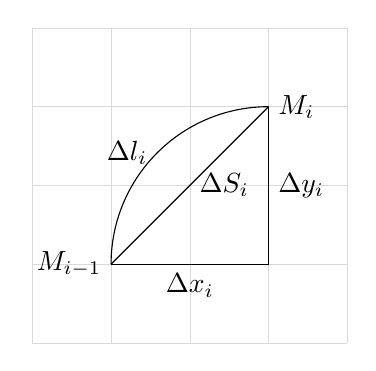
\begin{tikzpicture}
  
      \draw[very thin, gray!30, step = 1cm] (0, 0) grid (4, 4);
      \draw (1, 1) -- (3, 1) -- (3, 3);
      \draw (3, 3) arc (90:180:2) node[midway, above, left] {\(\Delta l_{i}\)};
      \draw (1, 1) -- (3, 3) node[midway, below, right] {\(\Delta S_{i}\)};

      \draw node[below] at (2, 1) {\(\Delta x_{i}\)};
      \draw node[right] at (3, 2) {\(\Delta y_{i}\)};
      \draw node[left] at (1, 1) {\(M_{i - 1}\)};
      \draw node[right] at (3, 3) {\(M_{i}\)};
    
    \end{tikzpicture}
  \end{multicols}

  \item Заметим, что \(\dfrac{\Delta y_{i}}{\Delta x_{i}}\) это отношение
  конечных приращений, поэтому можно применить т. Лагранжа:
  \begin{align*}
    \exists \xi_{i} \in [x_{i - 1}, x_{i}] \colon
      \frac{\Delta y_{i}}{\Delta x_{i}} = f'(\xi_{i})
    \\
    \Delta S_{i}
    = \sqrt{1 + y'(\xi_{i})^2} \Delta x_{i}
  \end{align*}
  
  \item Составим предел интегральных сумм и перейдем к интегралу:

  \begin{align*}
    S = \lim_{\substack{n \to \infty \\ \tau \to 0}}
      \sum_{i = 1}^{n} \sqrt{1 + y'(\xi_{i})^2} \Delta x_{i}
    \implies S = \int_{a}^{b} \sqrt{1 + y'(x)^2} \dd x
  \end{align*}
\end{enumerate}

\begin{remark}
  Выражение \(\dd l = \sqrt{1 + y'(x)^2} \dd x\) называется дифференциалом дуги.
\end{remark}
  \question{Решение ЛНУ\(_2\) с постоянными коэффициентами: специальная правая часть, поиск частного решения методом неопределенных коэффициентов.}


  \subsection{%
  Правила дифференцирования: производная сложной функции, инвариантность
  дифференциала.%
}

\begin{theorem}[Производная сложной функции]
  \begin{equation*}
    \begin{rcases}
      g(x) \isdiffd{x} \\
      f(g) \isdiffd{g_0 = g(x)}
    \end{rcases}
    \implies
    f'(g(x)) = f'(g) \cdot g'(x)
  \end{equation*}
\end{theorem}

\begin{proof}
  По критерию дифференцируемости имеем

  \begin{equation*} \label{eq:diff-cpx-func-1} \tag{1}
    \begin{aligned}
      u = g(x) \isdiffd{x}
      \implies
      \Delta u = g'(x) \Delta x + \smallo(\Delta x)
    \\
      y = f(g) \isdiffd{g_0}
      \implies
      \Delta y = f'(u) \Delta u + \smallo(\Delta u)
    \\
      \Delta y = f'(u)(g'(x) \Delta x + \smallo(\Delta x)) + \smallo(\Delta u)
    \end{aligned}
  \end{equation*}
  
  Также заметим, что 

  \begin{equation*} \label{eq:diff-cpx-func-2} \tag{2}
    u = g(x) \isdiffd{x} \implies g(x) \iscontd{x}
    \iff
    \Delta x \to 0 \implies \Delta u \to 0
  \end{equation*}

  Напишем определение производной для исходной функции.

  \begin{equation*} \label{eq:diff-cpx-func-3} \tag{3}
    \prh{f(g(x))}'
    = \lim_{\Delta x \to 0} \frac{\Delta y}{\Delta x}
    = \lim_{\Delta x \to 0} f'(u) g'(x)
      + f'(u) \frac{\smallo(\Delta x)}{\Delta x}
      + \frac{\smallo(\Delta u)}{\Delta x}
  \end{equation*}

  Второе и третье слагаемые в дают ноль в пределе, как отношение б.м. функции
  более высокого порядка и её аргумента (см. \eqref{eq:diff-cpx-func-2}), значит
  \(\prh{f(g(x)}' = f'(g) g'(x)\).
\end{proof}

\begin{remark}
  Если необходимо взять производную от композиции нескольких функций, то можно
  пользоваться \quote{расширенной} формулой производной композиции функций
  (правилом цепочки).

  \begin{equation*}
    \prh{f(g(h(\phi(x))))}' = f'(g) \cdot g'(h) \cdot h'(\phi) \cdot \phi'(x)
  \end{equation*}
\end{remark}

\begin{theorem}
  Первый дифференциал сохраняет инвариантность формы.
\end{theorem}

\begin{proof}
  Рассмотрим \(y = f(x)\), пусть \(x = u(t)\). Используя определение
  дифференциала и производную сложной функции получаем

  \begin{equation*}
    \dd y
    = y'_t \dd t
    = y'_x \cdot \under{x'_t \dd t}{\dd x}
    = y'_x \dd x
  \end{equation*}
  
  Таким образом, форма дифференциала не зависит от того, является аргумент
  функции независимой переменной или функцией другого аргумента.
\end{proof}

\begin{theorem}[Производная обратной функции]
  \begin{equation*}
    \begin{rcases}
      f(x) \isdiffd{x_0} \\
      f'(x_0) \neq 0 \\
      \exists g(y) = f^{-1}(y)
    \end{rcases}
    \implies
    g'(y) = \frac{1}{f'(x)}
  \end{equation*}
\end{theorem}

\begin{proof}
  Раскроем производную по определению и преобразуем.

  \begin{equation*} \label{eq:diff-inv-func-1} \tag{1}
    f'(x) = \lim_{\Delta x \to 0} \frac{\Delta y}{\Delta x}
    = \frac{1}{\lim_{\Delta x \to 0} \frac{\Delta x}{\Delta y}}
  \end{equation*}

  Заметим, что

  \begin{equation*} \label{eq:diff-inv-func-2} \tag{2}
    \begin{aligned}
      f(x) \isdiffd{x_0}
      \implies f(x) \iscontd{x_0}
      \iff \Delta x \to 0 \implies \Delta y \to 0
    \\
      \frac{1}{\lim_{\Delta x \to 0} \frac{\Delta x}{\Delta y}}
      = \frac{1}{\lim_{\Delta y \to 0} \frac{\Delta x}{\Delta y}}
    \end{aligned}
  \end{equation*}

  Выражение в знаменателе это и есть производная обратной функции. Таким образом
  из \eqref{eq:diff-inv-func-1} и \eqref{eq:diff-inv-func-2} следует, что

  \begin{equation*}
    f'(x)
    = \frac{1}{\lim_{\Delta y \to 0} \frac{\Delta x}{\Delta y}}
    = \frac{1}{g'(y)}
    \implies \prh{f^{-1}(y)}' = \frac{1}{f'(x)}
  \end{equation*}
\end{proof}

\begin{theorem}[Производная параметрически заданной функции]
  \begin{equation*}
    \begin{rcases}
      x = a(t) \isdiffd{t_0} \\
      y = b(t) \isdiffd{t_0} \\
      \exists a^{-1}(t) \\
      a'(t_0) \neq 0
    \end{rcases}
    \implies
    y'(x) = \frac{b'(t_0)}{a'(t_0)}
  \end{equation*}
\end{theorem}

\begin{proof}
  Т.к. \(a(t)\) обратима, то \(t = A(x)\), тогда по формуле производной сложной
  функции получаем

  \begin{equation*} \label{eq:diff-param-func-1} \tag{1}
    \prh{b(A(x))}'_x = b'_A \cdot A'_x
  \end{equation*}
  
  По формуле производной обратной функции \(\display{A'_x = \frac{1}{x'_A}}\).
  Учитывая, что \(A(x) = t\) и \(b(t) = y\), подставим это в
  \eqref{eq:diff-param-func-1}.

  \begin{equation*} \label{eq:diff-param-func-2} \tag{2}
    b(t)'_x = b'_t \cdot \frac{1}{x'_t} 
    \implies
    y'(x) = \frac{y'_t}{x'_t}
  \end{equation*}
\end{proof}
  \subsection{%
  Производные элементарных функций: константа, степенная функция.%
}

\begin{theorem}
  \begin{equation*}
    f(x) = c \implies f'(x) = 0
  \end{equation*}
\end{theorem}

\begin{proof}
  По определению производной

  \begin{equation*}
    f'(x) = \lim_{\Delta x \to 0} \frac{\Delta y}{\Delta x}
  \end{equation*}

  Т.к. \(f(x) = c\), то \(\Delta y = 0\), а значит

  \begin{equation*}
    f'(x) = \lim_{\Delta x \to 0} \frac{0}{\Delta x} = 0
  \end{equation*}
\end{proof}

\begin{theorem}
  \begin{equation*}
    f(x) = x^n \implies f'(x) = n x^{n - 1}
  \end{equation*}
\end{theorem}

\begin{proof}
  По определению производной
  
  \begin{equation*}
    f'(x)
    = \lim_{\Delta x \to 0} \frac{\Delta y}{\Delta x}
    = \lim_{\Delta x \to 0} \frac{f(x_0 + \Delta x) - f(x_0)}{\Delta x}    
  \end{equation*}

  Воспользуемся биномом Ньютона и вычислим полученную дробь.

  \begin{equation*}
    \begin{aligned}
      \frac{f(x_0 + \Delta x) - f(x_0)}{\Delta x}
    = \\
      \frac{(x_0 + \Delta x)^n - x_0^n}{\Delta x}
    = \\
      \frac{x_0^n + n x_0^{n - 1} \Delta x + \dotsc + (\Delta x)^n -
        x_0^n}{\Delta x}
    = \\
      \frac{n x_0^{n - 1} \Delta x + \dotsc + (\Delta x)^n}{\Delta x}
    = \\
      n x_0^{n - 1} + \dotsc + (\Delta x)^{n - 1}
    \end{aligned}
  \end{equation*}

  Заметим, что все слагаемые, кроме первого содержат \(\Delta x\), причем мы
  рассматриваем предел при \(\Delta x \to 0\). Это значит, что в пределе все
  слагаемые кроме первого обнулятся и получится

  \begin{equation*}
    f'(x)
    = \lim_{\Delta x \to 0} (n x_0^{n - 1} + \dotsc + (\Delta x)^{n - 1})
    = n x_0^{n - 1}
  \end{equation*}
\end{proof}

  \subsection{%
  Преобразование базиса и координат.%
}

\subheader{Переход к новому базису}

Пусть есть старый базис \(\set{\basis_i}_{i = 1}^n\) и новый базис
\(\set{\basis’_i}_{i = 1}^n\) и необходимо перейти от старого базиса к новому.
Разложим каждый из векторов старого базиса по новому базису.

\begin{equation*}
  \begin{cases}
    \basis_1 & = a_{1, 1} \basis'_1 + \dotsc + a_{1, n} \basis'_n \\
    \vdots & \\
    \basis_n & = a_{n, 1} \basis'_1 + \dotsc +  a_{n, n} \basis'_n 
  \end{cases}  
\end{equation*}

Теперь рассмотрим разложение произвольного вектора \(x\) в старом базисе.
Заменим в этом разложении каждый из векторов старого базиса на его разложение по
новому базису, перегруппируем и получим

\begin{equation*}
  \begin{aligned}
    x & = b_1 \basis_1 + \dotsc + b_n \basis_n  
  \\
    x & = b_1 (a_{1, 1} \basis'_1 + \dotsc + a_{1, n} \basis'_n)
      + \dotsc
      + b_n (a_{n, 1} \basis'_1 + \dotsc + a_{n, n} \basis'_n)
  \\
    x & = (b_1 a_{1, 1} + \dotsс + b_n a_{n, 1}) \basis'_1
    + \dotsc
    + (b_1 a_{1, n} + \dotsc + b_n a_{n, n}) \basis'_n
  \end{aligned}
\end{equation*}

\begin{remark}
  В матричном виде переход к новому базису можно выразить так

  \begin{equation*}
    B' = A^{-1 }B
  \end{equation*}

  А новые координаты можно вычислить так

  \begin{equation*}
    X_{B'} = A^T X_B
  \end{equation*}
\end{remark}

\subheader{Преобразования системы координат (СК)}

В качестве преобразований СК будет рассматривать только движения, причем будем
рассматривать движения именно СК, а не фигуры.

\begin{definition}
  Движение это отображение пространства в себя, которые сохраняет расстояние
  между точками.

  \begin{equation*}
    \begin{aligned}
      M(x, y) & \rarr{f} M'(x', y')
    \\
      O & \rarr{f} O'
    \\
      \abs{\vec{OM}} & = \abs{\vec{O'M'}}
    \end{aligned}
  \end{equation*}
\end{definition}

Существует несколько типов движений.

\begin{enumerate}
\item
  Осевая симметрия.
\item
  Параллельный перенос (сдвиг).
\item
  Поворот относительно точки.
\end{enumerate}

\subheader{Осевая симметрия}

\begin{definition}
  Осевой симметрией называется симметрия относительно одной (или нескольких) из
  осей.
\end{definition}

Координаты при этом меняются следующим образом.

\begin{equation*}
  \begin{array}{cc}
    \text{Симметрия относительно \(OY\)}
    &
    \text{Симметрия относительно \(OX\)}
  \\
    \begin{cases}
      x' = -x \\
      y' = y
    \end{cases}
    &
    \begin{cases}
      x' = x \\
      y' = -y
    \end{cases}
  \end{array}
\end{equation*}

\subheader{Параллельный перенос}

При параллельном переносе СК на вектор \(\vec{OO'}\) каждая точка переносится на
этот вектор. Перенос обозначается \(P_{\vec{a}}\), где \(\vec{a}\) это вектор
переноса.  

Координаты при этом меняются следующим образом:

\begin{equation*}
  \begin{cases}
    x = x' + x_0 \\
    y = y' + y_0
  \end{cases}
  \qquad
  \begin{cases}
    x' = x - x_0 \\
    y' = y - y_0
  \end{cases} 
\end{equation*}

где \((x_0, y_0)\) координаты точки \(O'\) в старой СК.

\begin{remark}
  При параллельном переносе направления осей сохраняются, т.е.
  \(OX \collinear O'X'\) и \(OY \collinear  O'Y'\).
\end{remark}

\subheader{Поворот СК}

Рассмотрим поворот СК \textbf{вокруг начала координат} на угол \(\alpha\)
\textbf{против часовой стрелки}.

Координаты при этом меняются следующим образом:

\begin{equation*} \label{eq:CS-rotate} \tag{ROT}
  \begin{cases}
    x = x' \cos \alpha - y' \sin \alpha \\
    y = x' \sin \alpha + y' \cos \alpha
  \end{cases}
  \qquad
  \begin{cases}
    x' = x \cos \alpha + y \sin \alpha \\
    y' = -x \sin \alpha + y \cos \alpha
  \end{cases}
\end{equation*}

\begin{remark}
  Матрица \(\display{\mtxp{
    \cos \alpha & -\sin \alpha \\
    \sin \alpha & \cos \alpha
  }}\)  называется матрицей поворота. Если умножить старые координаты на неё, то
  получатся новые координаты. Матрица обратного преобразования является обратной
  матрицей к матрице поворота. 
\end{remark}

\galleryone{01_19_01}{Смена координат при повороте СК}
 
Покажем, как можно получить формулы \eqref{eq:CS-rotate}.

\begin{proof}
  При повороте центр СК остается прежним и угол между осями не изменяется,
  значит \(O' = O\) и \(\angle(OX, OY) = \angle(OX', OY')\). Пусть
  \(\abs{\vec{a}} = \rho\), введём полярную СК (\(O\) полюс, \(OX\) полярная
  ось). Обозначим \((x, y)\) координаты вектора \(\vec{a}\) в старой СК, а
  \((x', y')\)~--- в новой. Из \figref{01_19_01} получаем

  \begin{align*}
    \begin{cases}
      x' = OB = \rho \cos (\omega - \alpha) \\
      y' = OA = \rho \sin(\omega - \alpha)
    \end{cases}
    \label{eq:CS-rotate-1} \tag{1}
  \\
    \begin{cases}
      x = OC = \rho \cos \omega \\
      y = OD = \rho \sin \omega
    \end{cases}
    \label{eq:CS-rotate-2} \tag{2}
  \end{align*}

  В \eqref{eq:CS-rotate-1} применим тригонометрические формулы.

  \begin{equation*} \label{eq:CS-rotate-3} \tag{3}
    \begin{cases}
      x' = \under{\rho \cos \omega}{x} \cos \alpha
        + \under{\rho \sin \omega}{y} \sin \alpha
      \\
      y' = \under{\rho \sin \omega}{y} \cos \alpha
        - \under{\rho \cos \omega}{x} \sin \alpha
    \end{cases}
  \end{equation*}

  Подставим \eqref{eq:CS-rotate-2} в \eqref{eq:CS-rotate-3}.

  \begin{equation*}
    \begin{cases}
      x' = x \cos \alpha + y \sin \alpha \\
      y' = y \cos \alpha - x \sin \alpha
    \end{cases}
    \implies
    \begin{cases}
      x' = x \cos\alpha + y \sin \alpha \\
      y' = -x \sin \alpha + y \cos \alpha
    \end{cases}
  \end{equation*}
\end{proof}

  \question{Виды векторных полей и их свойства (теоремы о поле градиента и поле вихря).}


  \question{Механический смысл потока и дивергенции.}


  \question{Признаки сходимости несобственных интегралов: второй признак сравнения (предельный).}


  \subsection{Теоремы о дифференцируемых функциях. Теорема Ферма.}

  \subsection{%
  Теоремы о дифференцируемых функциях. Теорема Ролля.%
}

\begin{theorem}[Ролля]
 \begin{equation*}
  \begin{rcases}
    f(x) \isdiff{\segment{a}{b}} \\
    f(a) = f(b)
  \end{rcases}
  \implies \exists \xi \in \interval{a}{b} \given f'(\xi) = 0
 \end{equation*}
\end{theorem}

\begin{proof}  
  Т.к. функция дифференцируема на отрезке, то она непрерывна на этом отрезке,
  значит по второй теореме Вейерштрасса она принимает наибольшее и наименьшее
  значения на этом отрезке (\(M\) и \(m\)). Если наибольшее или наименьшее
  значения достигаются на концах отрезка, то \(f(a) = f(b) = M = m\). Значит по
  второй теореме Больцано-Коши функция принимает все значения от \(m\) до \(M\),
  т.е. является константой. Таким образом её производная равна нулю в любой
  точке отрезка.

  Если наибольшее или наименьшее значения достигаются внутри, то это означает,
  что внутри отрезка у функции есть экстремум. Таким образом, по лемме Ферма,
  если функция дифференцируема в точке и при этом в этой точке достигается
  экстремум, то производная в этой точке равна нулю. В обоих случаях нашлась
  некоторая точка, производная в которой равна нулю.
\end{proof}

Геометрический смысл теоремы Ролля заключается в том, что она говорит о смене
монотонности функции (\figref{01_24_01}).

\galleryone{01_24_01}{Геометрический смысл теоремы Ролля}

\end{questions}

\newpage
\section{Интегрирование функции нескольких переменных}

\begin{questions}
  \question{Обыкновенное дифференциальное уравнение (ДУ): задача о радиоактивном распаде и задача о падении тела. Определение ДУ, решения ДУ и их геометрический смысл. Задача Коши.}

\begin{definition}
  Обыкновенным ДУ\(_{n}\) называется

  \begin{align*}
    F(x, y, \dotsc, y^{(n)}) = 0
  \end{align*}
\end{definition}

\begin{remark}
  'Обыкновенное' означает не в частных дифференциалах, т.е. \(y(x)\) это
  функция одно переменной.
\end{remark}

\begin{definition}
  Порядком ДУ называется наивысший порядок входящей в него производной.
\end{definition}

\begin{definition}
  Решением ДУ\(_{n}\) является функция, которая обращает его в верное равенство.
\end{definition}

\begin{definition}
  Кривые, соответствующие решениям ДУ называются интегральными кривыми.
\end{definition}

\begin{definition}
  Если решение ДУ задано неявно \(\phi(x, y(x)) = 0\), то 
  \(\phi(x, y(x)) = 0\) называется интегралом ДУ.
\end{definition}

\begin{definition}
  Решение ДУ с неопределенными константами \(c_{i}\) называется общим решением
  (общим интегралом) ДУ.  
\end{definition}

\begin{definition}
  Решение ДУ с определенными константами \(c_{i}\) называется частным решением
  (частным интегралом) ДУ.
\end{definition} 

\begin{definition}
  Система из ДУ\(_{n}\) и \(n\) начальных условий вида

  \begin{align*}
    \begin{cases}
      \text{ДУ}_n \\
      y_0 = y(x_0) \\
      y'_0 = y'(x_0) \\
      \dots \\
      y^{(n - 1)}_0 = y^{(n - 1)}(x_0)
    \end{cases}
  \end{align*}

  называется задачей Коши. \(n\) начальных условий необходимы для определения
  \(n\) констант \(c_{i}\).
\end{definition}

\begin{remark}
  Подробнее про задачу Коши и геометрический смысл решений рассказано в
  \ref{ex-un-Cp}.
\end{remark}

\underline{Задача о радиоактивном распаде}: 

Пусть есть \(Q\) грамма урана, скорость распада которого зависит от его массы с
некоторым коэффициентом \(k\). Требуется вывести формулу для подсчета массы
урана в момент времени \(t\).

Составим ДУ и решим его:

\begin{align*}
  \frac{\dd Q}{\dd t} = -k Q \mid \colon Q \neq 0
  \\
  \frac{\dd Q}{Q \dd t} = -k
  \iff
  \frac{\dd \ln Q}{\dd t} + k = 0
  \\
  \frac{\dd \ln Q + k \dd t}{\dd t} = 0
  \iff
  \frac{\dd (\ln Q + k t)}{\dd t} = 0
  \\
  \ln Q + kt = c_{1} \\
  Q = \widehat{c_{1}} e^{-k t}
\end{align*}

Из полученных интегральных кривых выбираем одну, которая соответствует
заданным начальным условиям.

\underline{Задача о падении тела}: 

Тело свободно падает вниз с заданной начальной скоростью. Требуется вывести
закон движения (закон изменения координат с течением времени).

Составим ДУ и решим его:

\begin{align*}
  \vec{F} = m \vec{a} = m \vec{g} \implies a = y''(t) = g \\
  \frac{\dd^{2} y(t)}{\dd t^{2}} = g
  \implies \frac{\dd v(t)}{\dd t} = g 
  \implies v(t) = g t + c_{1} \\
  \frac{\dd y(t)}{\dd t}  = v(t) = g t + c_{1}
  \implies y(t) = \frac{g t^{2}}{2} + c_{1} t + c_{2}
\end{align*}

Как и в первой задаче здесь получено общее решение. Константы можно найти
подстановкой начальных условий.

  \question{Замена переменной в неопределенном интеграле. Интегрирование по частям.}

\begin{remark}
  Интеграл сохраняет инвариантность своей формы, т.е.

  \begin{align*}
    \int f(\clubsuit) \dd \clubsuit = F(\clubsuit) + C
  \end{align*}
\end{remark}

\begin{theorem}\label{ad-rep}
  О замене производной в неопределенном интеграле

  Если \(x = \phi(t)\), где \(\phi(t)\) обратимая и дифференцируемая
  функция, то

  \begin{align*}
    \int f(x) \dd x = \int f(\phi(t)) \phi'(t) \dd t
  \end{align*}
\end{theorem}
\begin{proof}
  Возьмем производные от обоих частей:

  \begin{align*}
    \left( \int f(x) \dd x \right)'_{x} = f(x) \\
    \left( \int f(\phi(t)) \phi'(t) \dd t \right)'_{x} =
    \left( \int f(\phi(t)) \phi'(t) \dd t \right)'_{t} \frac{\dd t}{\dd x}
    \transition{\ref{ad-prop-2}}
    f(\phi(t)) \phi'(t) \frac{\dd t}{\dd x} =
    f(\phi(t)) \phi'(t) \frac{1}{\phi'(t)} =
    f(\phi(t)) =
    f(x)
  \end{align*}
\end{proof}

\begin{remark}
  Формула работает в обе стороны:

  \begin{align*}
    \int \frac{e^{\sqrt{x}}}{\sqrt{x}} \dd x
    \transition{\sqrt{x} = t}
    \int \frac{e^{t}}{t} 2t \dd t =
    2 e^{t} + C =
    2 e^{\sqrt{x}} + C
  \end{align*}

  \begin{align*}
    \int e^{x^{2}} \underbrace{2x \dd x}_{\dd x^2}
    \transition{x^2 = t}
    \int e^{t} \dd t =
    e^{t} + C =
    e^{x^2} + C
  \end{align*}
\end{remark}

\begin{theorem}
  Интегрирование по частям

  \begin{align*}
    \int u \dd v = u v - \int v \dd u
  \end{align*}
\end{theorem}
\begin{proof}
  Рассмотрим равенство \((u v)' = u' v + u v'\) и проинтегрируем обе его части:

  \begin{align*}
    (u v)' = u' v + u v'
    \\
    \int (u v)' \dd x = \int u' v + u v' \dd x
    \\
    u v = \int u' v \dd x + \int u v' \dd x
      \tag*{Линейность интеграла (\ref{ad-prop-3})}
    \\
    u v = \int v \dd u + \int u \dd v
      \tag*{Внесение под дифференциал (\ref{ad-rep})}
    \\
    \int u \dd v = u v - \int u \dd v
  \end{align*}
\end{proof}

\begin{remark}
  Интегрирование по частям используется если \(\int v \dd u\) вычисляется проще,
  чем интеграл \(\int u \dd v\). В качестве функции \(u\) выбирают ту, которая
  упрощается при дифференцировании.
\end{remark}

  \question{Детерминированный конечный автомат.}

Детерминированный конечный автомат (ДКА) это кортеж вида
\(\Tuple{\Sigma, Q, q_{0}, F, \delta}\), где
\begin{itemize}
  \item \(\Sigma\) это алфавит
  \item \(Q\) это множество состояний
  \item \(q_{0}\) это начальное состояние (\(q_{0} \in Q\))
  \item \(F\) это множество принимающих состояний (\(F \subseteq Q\))
  \item \(\delta\) это функция перехода \(\delta \colon Q \times \Sigma \to Q\)
\end{itemize}

Мы рассматриваем только автоматы-детекторы, т.е. им на вход подается слово,
после обработки которого автомат оказывается в одном из состояний. Если это
принимающее состояние, то говорят, что слово принимается автоматом (автомат
допускает слово), в противном случае~--- слово отвергается автоматом.

\underline{Вычисление}:

\begin{definition}
  Снимок (\textit{snapshot}) это упорядоченная пара вида \(\Pair{q, s}\), где
  \(q \in Q\) это текущее состояние, а \(s\) это еще непросмотренная часть входной
  строки.
\end{definition}

Множество всех снимков обозначается \(SNAP\). На этом множество можно ввести
бинарное отношение \(\vdash\), которое будет показывать, можно ли перейти от
одного снимка к другому:

\begin{align*}
  \Pair{q_{1}, s_{1}} \vdash \Pair{q_{2}, s_{2}}
  \iff
  \begin{cases}
    s_{1} = \alpha s_{2} \\
    \delta(q_{1}, \alpha) = q_{2}
  \end{cases}
\end{align*}

\begin{definition}
  Автоматный язык \(\Lang(\mathcal{A})\) это язык, состоящий из слов,
  принимаемых автоматом:

  \begin{align*}
    \Lang(\mathcal{A})
    = \{ s \mid \Pair{a_{0}, s} \vdash^{*} \Pair{f, \epsilon}, f \in F \}
  \end{align*}
\end{definition}

\begin{definition}
  Множество автоматных языков \(AUT\) это множество языков, для которых
  существует автомат их принимающий.

  \begin{align*}
    AUT = \{
      \mathcal{X} \mid \exists \mathcal{A} \colon
      \Lang(\mathcal{A}) = \mathcal{X}
    \}
  \end{align*}
\end{definition}

  \question{Композиции.}

\begin{definition}
  Слабой композицей числа \(n \ge 0\) на \(k\) частей называется решение
  уравнения \(b_{1} + \dotsc + b_{k} = n\) при условии \(b_{i} \ge 0\).
\end{definition}

Для подсчета числа слабых композиций воспользуемся методом Stars\&Bars: пусть у
нас есть \(n\) единиц и \(k - 1\) перегородка между ними, значит всего получаем

\begin{align*}
  \Big|
    \text{Количество слабых композиций } n \text{ на } k \text{ частей}
  \Big|= \binom{n + k - 1}{k - 1}
\end{align*}

\begin{definition}
  Композицией числа \(n \ge 0\) на \(k\) частей называется решение уравнения
  \(b_{1} + \dotsc + b_{k} = n\) при условии \(b_{i} \ge 0\).
\end{definition}

Количество композиций числа можно посчитать следующим образом: возьмем из \(n\)
\(k\) единиц (по одной для каждого слагаемого), а для оставшихся \(n - k\)
единиц решим задачу о слабой композиции. Итого получим

\begin{align*}
  \Big|
    \text{Количество композиций } n \text{ на } k \text{ частей}
  \Big| = \binom{n - 1}{k - 1}
\end{align*}

\begin{remark}
  Число композиций числа \(n\) на произвольное число частей
  (т.е. \(k = 1 \dots n\)) равно \(2^{n - 1}\).
\end{remark}

  \subsection{%
  Предельный переход в неравенствах. Теорема о двух милиционерах.%
}

\begin{theorem} \label{thr:lim-func}
  Если функция \(f(x)\) имеет предел в точке \(a\), то она ограничена в
  некоторой проколотой окрестности этой точки.
\end{theorem}

\begin{proof}
  Раскроем модуль в определении предела.

  \begin{equation*}
    \begin{aligned}
      \lim_{x \to a} f(x) = L \iff
      \forall \epsilon > 0 \exists \delta > 0 \given
      \forall x \in \nearo{a}{\delta} \cap E \implies
      \abs{f(x) - L} < \epsilon
    \\
      L - \epsilon < f(x) < L + \epsilon
    \end{aligned}
  \end{equation*}

  Получается, что функция \(f(x)\) ограничена в проколотой окрестности точки
  \(a\).
\end{proof}

\begin{theorem}[О стабилизации знака] \label{thr:stable-sign}
  Если \(\lim_{x \to a} f(x) = A > 0\), то \(f(x) > 0\) в некоторой окрестности
  \(a\).
\end{theorem}

\begin{proof}
  По теореме \ref{thr:lim-func}, получаем, что \(f(x)\) ограничена в некоторой
  проколотой \(\epsilon\)--окрестности точки \(a\), т.е. \(A - \epsilon < f(x)
  < A + \epsilon\). Пусть \(\epsilon = \frac{A}{2}\), тогда \(f(x) > A -
  \frac{A}{2} > 0\).
\end{proof}

\begin{theorem}[О предельном переходе в неравенствах]
  Если \(f(x) \le g(x)\) в некоторой окрестности точки \(a\), то 
  
  \begin{equation*}
    \begin{rcases}
      \lim_{x \to a} f(x) = A \\
      \lim_{x \to a} g(x) = B
    \end{rcases}
    \implies
    A \le B
  \end{equation*}
\end{theorem}

\begin{proof}
  От противного: пусть \(A > B\), тогда

  \begin{equation*}
    \lim_{x \to a} f(x) - \lim_{x \to a} g(x)
    = \lim_{x \to a} (f(x) - g(x))
    = A - B > 0
  \end{equation*}

  Тогда по \ref{thr:stable-sign} \(f(x) - g(x) > 0\), т.е. \(f(x) > g(x)\) в
  некоторой проколотой \(\delta_1\)--окрестности точки \(a\). По условию \(f(x)
  \le g(x)\) в некоторой \(\delta_2\)-окрестности точки \(a\). Пусть \(\delta =
  \min(\delta_1, \delta_2)\), тогда по свойству окрестностей оба условия должны
  выполняться, т.е. \(f(x) \le g(x)\) и \(f(x) > g(x)\). Противоречие.
\end{proof}

\begin{theorem}[О двух милиционерах] \label{thr:squeezed-func}
  Если \(f(x) \le h(x) \le g(x)\) в некоторой проколотой окрестности точки
  \(a\), то

  \begin{equation*}
    \begin{rcases}
      \lim_{x \to a} f(x) = A \\
      \lim_{x \to a} g(x) = A
    \end{rcases}
    \implies
    \lim_{x \to a}h(x) = A
  \end{equation*}
\end{theorem}

\begin{proof}
  Запишем условие формально, раскрыв два предела по определению

  \begin{equation*}
    \begin{aligned}
      \lim_{x \to a} f(x)  = A \iff
      \forall \epsilon > 0 \exists \delta_1 > 0 \given
      \forall x \in \nearo{a}{\delta_1} \cap X \implies
      \abs{f(x) - A} < \epsilon
    \\
      \lim_{x \to a} g(x) = A \iff
      \forall \epsilon > 0 \exists \delta_2 > 0 \given
      \forall x \in \nearo{a}{\delta_2} \cap X \implies
      \abs{g(x) - A} < \epsilon
    \\
      \exists \delta_3 > 0 \given
      \forall x \in \nearo{a}{\delta_3} \cap X \colon
      f(x) \le h(x) \le g(x)
    \end{aligned}
  \end{equation*}

  Пусть \(\delta = \min(\delta_1, \delta_2, \delta_3)\), тогда по свойству
  окрестностей все условия будут выполняться. Раскроем модули по определению и
  \quote{склеим} полученные неравенства.

  \begin{equation*}
    \begin{rcases}
      A - \epsilon < f(x) < A + \epsilon \\
      A - \epsilon < g(x) < A + \epsilon
    \end{rcases}
    \implies
    A - \epsilon < f(x) \le h(x) \le g(x) < A + \epsilon
    \implies
    A - \epsilon < h(x) < A + \epsilon
  \end{equation*}

  Причем последнее неравенство выполняется в проколотой окрестности точки \(a\)
  для любого \(\epsilon\). Таким образом \(\lim_{x \to a} f(x) = A\) по
  определению предела.
\end{proof}

Теорема \ref{thr:squeezed-func} также называется теоремой о двух жандармах или
теоремой о сжатой функции.

  \question{Двудольные графы.}

\begin{definition}
  Двудольный граф это граф, вершины которого могут быть разбиты на два множества
  (две доли) так, что между вершинами каждого из множеств не будет ребер.
\end{definition}

\begin{remark}
  Об обозначениях.

  Двудольный граф обычно обозначается как \(G = \Triple{X, Y, E}\), где \(X\) и
  \(Y\) это его доли, а \(E\)~---- множество ребер между этими долями.

  Пусть задано некоторое подмножество \(S \subseteq X\), тогда \(E(S)\) это
  множество ребер, инцидентных вершинам из множества \(S\).

  Обозначение \(N(S)\) используется что показать 'соседей' для вершин из
  множества \(S\), т.е. такие вершины из множества \(Y\), которые смежны хотя
  бы с одной из вершин из множества \(S\).
\end{remark}

\begin{definition}
  Двудольный граф называется сбалансированным, если размеры его долей совпадают.
\end{definition}

\begin{theorem}\label{bipartite-balance}
  \(r\)-регулярный двудольный граф является сбалансированным.
\end{theorem}
\begin{proof}
  Пусть дан двудольный граф \(G = \Triple{X, Y, E}\).
  Т.к. он двудольный, то множество ребер может быть представлено в виде
  \(\abs{E} = \abs{X} \cdot r\). С другой стороны оно может быть представлено в
  виде \(\abs{E} = \abs{Y} \cdot r\). Приравниваем и получаем искомое равенство
  \(\abs{X} = \abs{Y}\).
\end{proof}

\begin{theorem}
  В любом регулярном двудольном графе существует совершенное паросочетание.
\end{theorem}
\begin{twocolumns}
  \begin{proof}
    Рассмотрим двудольный граф \(G = \Triple{X, Y, E}\). Выберем произвольное
    \(S \subseteq X\). Заметим, что \(E(N(S)) \ge E(S)\), причем т.к. граф
    регулярный, то \(E(N(S)) = \abs{N(S)} \cdot r\), а
    \(E(S) = \abs{S} \cdot r\).

    Подставляя это в полученное ранее неравенство, получаем, что
    \(\abs{N(S)} \ge \abs{S}\) причем это выполняется для любого
    \(S \subseteq X\). Значит по т. Холла (\ref{Hall}) в графе существует
    \(X\)-совершенное паросочетание.

    Т.к. \(G\)~--- регулярный двудольный граф, то по \ref{bipartite-balance} он
    сбалансирован, значит \(\abs{X} = \abs{Y}\). Таким образом \(X\)-совершенное
    паросочетание является совершенным паросочетанием.
  \end{proof}
  \columnbreak

  \begin{figure}[H]
  \centering

  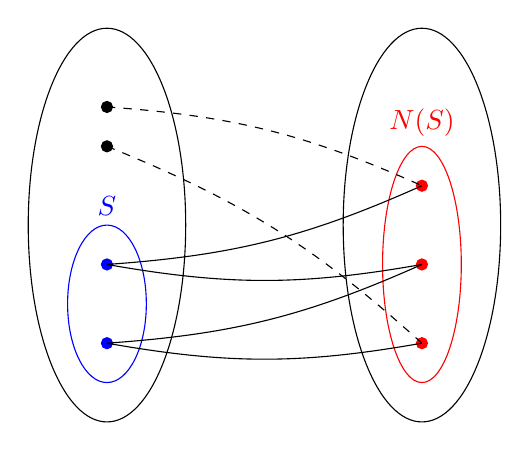
\begin{tikzpicture}
    \coordinate (L1) at (-2, -0.5);
    \coordinate (L2) at (-2, -1.5);

    \coordinate (LS1) at (-2, 1.5);
    \coordinate (LS2) at (-2, 1);

    \coordinate (R1) at (2, 0.5);
    \coordinate (R2) at (2, -0.5);
    \coordinate (R3) at (2, -1.5);

    \draw (-2, 0) ellipse (1cm and 2.5cm);
    \draw (2, 0) ellipse (1cm and 2.5cm);

    \begin{scope}[every path/.style = {color = blue}]
      \draw (-2, -1) ellipse (0.5cm and 1cm);
      \draw node[above] at (-2, 0) {\(S\)};
      \draw[fill = blue] (L1) circle (2pt);
      \draw[fill = blue] (L2) circle (2pt);
    \end{scope}

    \draw[fill = black] (LS1) circle (2pt);
    \draw[fill = black] (LS2) circle (2pt);

    \begin{scope}[every path/.style = {color = red}]
      \draw (2,-0.5) ellipse (0.5cm and 1.5cm);
      \draw node[above] at (2, 1) {\(N(S)\)};
      \draw[fill = red] (R1) circle (2pt);
      \draw[fill = red] (R2) circle (2pt);
      \draw[fill = red] (R3) circle (2pt);
    \end{scope}

    \draw (L1) edge[bend right = 10] (R1);
    \draw (L1) edge[bend right = 10] (R2);
    \draw (L2) edge[bend right = 10] (R2);
    \draw (L2) edge[bend right = 10] (R3);

    \draw[dashed] (LS1) edge[bend left = 10] (R1);
    \draw[dashed] (LS2) edge[bend left = 10] (R3);
  \end{tikzpicture}  
\end{figure}
\end{twocolumns}

  \question{Интегрирование некоторых иррациональных функций, метод тригонометрической подстановки.}

\begin{itemize}
\item Интегралы вида \(\int R(\sqrt{x^2 \pm 1}, x) \dd x\) решаются с помощью
замены \(x\) на гиперболическую функцию:

\begin{align*}
  \sinh u = \frac{e^u - e^{-u}}{2} \qquad
  \cosh u = \frac{e^u + e^{-u}}{2}
\end{align*}

Данные функции называются гиперболическим синусом и гиперболическим косинусом
соответственно.

\begin{lemma}
  Основное гиперболическое тождество

  \begin{align*}
    \cosh^2 u - \sinh^2 u = 1
  \end{align*}
\end{lemma}
\begin{proof}
  \begin{align*}
    \cosh^2 u - \sinh^2 u=
    \left(\frac{e^{u} + e^{-u}}{2}\right)^2
      - \left(\frac{e^{u} - e^{-u}}{2}\right)^2 =
    \frac{1}{4} \left(e^{2u} + 2 + e^{-2u} - e^{2u} + 2 - e^{-2u} \right) = 1
  \end{align*}
\end{proof}

\begin{remark}\label{hpr-rep}
  Заметим, что

  \begin{align*}
    \ln \abs{\sinh u + \cosh u}
    = \ln \abs{\frac{e^u - e^{-u}}{2} + \frac{e^u + e^{-u}}{2}}
    = \ln e^{u}
    = u
  \end{align*}
\end{remark}

\begin{example}
  Вычислим 'длинный' логарифм:

  \begin{align*}
    \int \frac{\dd x}{\sqrt{1 + x^2}} = 
    \begin{bmatrix}
      x = \sinh u \implies 1 + x^2 = \cosh^2 u \\
      \dd x = \dd (\sinh u) = \cosh u \dd u \\
      u = \ln \abs{
        \under{x}{\sinh u} + \under{\sqrt{1 + x^2}}{\cosh u}
      } \;\; (\ref{hpr-rep})
    \end{bmatrix} =
    \int \frac{\cosh u}{\cosh u} \dd u =
    u + C =
    \ln \abs{x + \sqrt{1 + x^2}} + C
  \end{align*}
\end{example}

\item Интегралы вида \(\int R(\sqrt{1 - x^2}, x) \dd x\) решаются с помощью
замены \(x\) на синус или косинус.

\item Интегралы вида \(\int R(\sqrt[k_{1}]{x}, \dots, \sqrt[k_{n}]{x}) \dd x\)
решаются с помощью замены \(t = \sqrt[K]{x}\), где \(K\) это НОК для
\(k_{1}, \dotsc, k_{n}\).

\item Интегралы вида \(\int R(\sqrt{ax + b}, x) \dd x\) решаются с помощью
замены \(t = \sqrt{ax + b}\). При этом \(x = \frac{t^2 - b}{a}\),
\(\dd x = \frac{2t}{a} \dd t\).
\end{itemize}

  \subsection{%
  Сравнение бесконечно малых. Теоремы об эквивалентных функциях.%
}

Пусть \(\infsmall_1(x)\) и \(\infsmall_2(x)\)~--- б.м. в точке \(a\), тогда

\begin{enumerate}
\item
  \(
    \lim_{x \to a} \frac{\infsmall_1(x)}{\infsmall_2(x)} = 0
    \implies \infsmall_1(x)
  \) более высокого порядка, чем \(\infsmall_2(x)\).

\item
  \(
    \lim_{x \to a} \frac{\infsmall_1(x)}{\infsmall_2(x)} \in \RR \setminus
    \set{0} \implies \infsmall_1(x)
  \) и \(\infsmall_2(x)\) одного порядка.

\item
  \(
    \lim_{x \to a} \frac{\infsmall_1(x)}{\infsmall_2(x)} = \infty
    \implies \infsmall_1(x)
  \) более низкого порядка, чем \(\infsmall_2(x)\).

\item
  \(
    \lim_{x \to a} \frac{\infsmall_1(x)}{\infsmall_2(x)^k} \in \RR \setminus
    \set{0} \implies \infsmall_1(x)
  \) имеет порядок \(k\) по отношению к \(\infsmall_2(x)\).
\end{enumerate}

Пусть \(\infbig_1(x)\) и \(\infbig_2(x)\)~--- б.б. в точке \(a\), тогда

\begin{enumerate}
\item
  \(
    \lim_{x \to a} \frac{\infbig_1(x)}{\infbig_2(x)} = 0
    \implies \infbig_1(x)
  \) более низкого порядка, чем \(\infbig_2(x)\).

\item
  \(
    \lim_{x \to a} \frac{\infbig_1(x)}{\infbig_2(x)} \in \RR \setminus
    \set{0} \implies \infbig_1(x)
  \) и \(\infbig_2(x)\) одного порядка.

\item
  \(
    \lim_{x \to a} \frac{\infbig_1(x)}{\infbig_2(x)} = \infty
    \implies \infbig_1(x)
  \) более высокого порядка, чем \(\infbig_2(x)\).

\item
  \(
    \lim_{x \to a} \frac{\infbig_1(x)}{\infbig_2(x)^k} \in \RR \setminus
    \set{0} \implies \infbig_1(x)
  \) имеет порядок \(k\) по отношению к \(\infbig_2(x)\).
\end{enumerate}

\begin{remark}
  \(\smallo(f(x))\)~--- обозначение б.м. более высокого порядка для функции
  \(f(x)\). Обычно это обозначение используют для сравнения с некоторым эталоном
  \(\Delta x\), например

  \begin{equation*}
    \infsmall(x) = \smallo(\Delta x)
    \iff
    \lim_{x \to a} \frac{\infsmall(x)}{\Delta x} = 0
  \end{equation*}
\end{remark}

\begin{remark}
  Таким образом, разрешение неопределенностей вида
  \(\display{\left[\frac{0}{0}\right]}\) и
  \(\display{\left[\frac{\infty}{\infty}\right]}\) это на самом деле сравнение
  бесконечно малых и бесконечно больших функций.
\end{remark}

\begin{definition}
  Если \(\lim_{x \to a} \frac{\infsmall_1(x)}{\infsmall_2(x)} = 1\), то
  \(\infsmall_1(x)\) и \(\infsmall_2(x)\) называются эквивалентными б.м.
  функциями.

  \begin{equation*}
    \lim_{x \to a} \frac{\infsmall_1(x)}{\infsmall_2(x)} = 1
    \iff
    \infsmall_1(x) \sim \infsmall_2(x)
  \end{equation*}
\end{definition}

\begin{remark}
  Геометрический смысл эквивалентных функций заключается в том, что в малой
  окрестности точки \(a\) графики функций сливаются. В качестве примера можно
  рассмотреть функции \(\sin x\) и \(x\) (\figref{01_08_01}).
\end{remark}

\galleryone{01_08_01}{Эквивалентные функции}

\begin{theorem}
  В произведении можно заменять эквивалентные функции друг на друга при
  условии, что они эквивалентны \textbf{в одной точке}.

  \begin{equation*}
    \alpha(x) \sim \gamma(x)
    \implies
    \lim_{x \to a} \frac{\infsmall(x)}{\beta(x)}
    = \lim_{x \to a} \frac{\gamma(x)}{\beta(x)}
  \end{equation*}
\end{theorem}

\begin{proof}
  Домножим на \(\gamma(x)\) и воспользуемся свойством произведения пределов.

  \begin{equation*}
    \lim_{x \to a} \frac{\alpha(x)}{\beta(x)} 
    = \lim_{x \to a} \frac{\alpha(x) \cdot \gamma(x)}{\beta(x) \cdot \gamma(x)}
    = \lim_{x \to a} \frac{\alpha(x)}{\gamma(x)} \cdot
      \lim_{x \to a} \frac{\gamma(x)}{\beta(x)}
  \end{equation*}

  По определению эквивалентных функций левый предел равен единице, значит

  \begin{equation*}
    \lim_{x \to a} \frac{\alpha(x)}{\beta(x)}
    = \lim_{x \to a} \frac{\gamma(x)}{\beta(x)}
  \end{equation*}
\end{proof}

\begin{theorem}
  Разность эквивалентных \textbf{в одной точке} б.м. функций это б.м. более
  высокого порядка, чем эти функции.

  \begin{equation*}
    \alpha(x) \sim \beta(x)
    \implies
    \alpha(x) - \beta(x) = \smallo(\alpha(x)) = \smallo(\beta(x))
  \end{equation*}
\end{theorem}

\begin{proof}
  Сравним \(\alpha(x) - \beta(x)\) по определению сравнения б.м. функций, для
  этого вычислим следующий предел

  \begin{equation*}
    \lim_{x \to a} \frac{\alpha(x) - \beta(x)}{\alpha(x)}
    = \lim_{x \to a} 1 - \frac{\beta(x)}{\alpha(x)}
    = 1 - \lim_{x \to a} \frac{\beta(x)}{\alpha(x)}
  \end{equation*}

  По определению эквивалентных функций правый предел равен единице, значит

  \begin{equation*}
    \lim_{x \to a} \frac{\alpha(x) - \beta(x)}{\alpha(x)}
    = 1 - 1
    = 0
  \end{equation*}

  Таким образом \(\alpha(x) - \beta(x)\) это б.м. более высокого порядка, чем
  \(\alpha(x)\). Для \(\beta(x)\) доказательство аналогично.
\end{proof}

\begin{theorem}
  Произведение двух б.м. \textbf{в одной точке} функций это б.м. более высокого
  порядка, чем эти функции.

  \begin{equation*}
    \alpha(x) \cdot \beta(x) = \smallo(\alpha(x)) = \smallo(\beta(x))
  \end{equation*}
\end{theorem}

\begin{proof}  
  Сравним \(\alpha(x) \cdot \beta(x)\) по определению сравнения б.м. функций,
  для этого вычислим следующий предел

  \begin{equation*}
    \lim_{x \to a} \frac{\alpha(x) \cdot \beta(x)}{\alpha(x)}
    = \lim_{x \to a} \beta(x)
  \end{equation*}

  По определению б.м. функции этот предел равен нулю. Таким образом \(\alpha(x)
  \cdot \beta(x)\) это б.м. более высокого порядка, чем \(\alpha(x)\). Для
  \(\beta(x)\) доказательство аналогично.
\end{proof}

  \question{Геометрический смысл определенного интеграла. Оценка определенного интеграла. Теорема о среднем.}


  \question{Структура образа самосопряженного оператора. Проектор. Спектральное разложение оператора.}

\begin{theorem}\label{sconj-lo-img}
  Образ самосопряженного оператора \(\opA \colon V^{n} \to V^{n}\) имеет вид

  \begin{align*}
    \Img \opA = \left\{
      \sum_{i = 1}^{n}
      \lambda_{i} (x, \basis_{i}) \basis_{i}
      \mid x \in V^{n}
    \right\}
  \end{align*}

  где \(\Basis = \{ \basis_{i} \}_{i = 1}^{n}\) это ортонормированный базис,
  \(\lambda_{i}\)~--- собственные числа оператора \(\opA\).
\end{theorem}
\begin{proof}
  \begin{align*}
    \opA x = y =
    \\
      y_{1} \basis_{1}
        + \dotsc + y_{n} \basis_{n} =
    \\
      (y, \basis_{1}) \basis_{1}
        + \dotsc + (y, \basis_{n}) \basis_{n} =
    \\
      (\opA x, \basis_{1}) \basis_{1}
        + \dotsc + (\opA x, \basis_{n}) \basis_{n} =
    \\
      (x, \opA \basis_{1}) \basis_{1}
        + \dotsc + (x, \opA \basis_{n}) \basis_{n} =
    \\
      (x, \lambda_{1} \basis_{1}) \basis_{1}
        + \dotsc + (x, \lambda_{n} \basis_{n}) \basis_{n} =
    \\
      \lambda_{1} (x, \basis_{1}) \basis_{1}
        + \dotsc + \lambda_{n} (x,\basis_{n}) \basis_{n} =
    \\
    \sum_{i = 1}^{n} \lambda_{i} (x, \basis_{i}) \basis_{i}
  \end{align*}
\end{proof}

\begin{remark}
  \((x, \basis_{i})\) это проекция вектора \(x\) на собственный вектор.

  Таким образом \(y\) получается следующим образом: \(x\) проецируется на 
  \(\basis_{1}, \dotsc, \basis_{n}\), после чего проекции 'растягиваются' в
  \(\lambda_{1}, \dotsc, \lambda_{n}\) раз и суммируются.
\end{remark}

\begin{definition}\label{lo-proj}
  Оператор вида

  \begin{align*}
    P_{i}(x) = (x, \basis_{i}) \basis_{i}
  \end{align*}

  называется проектором на одномерное пространство, порожденное собственным
  вектором.
\end{definition}

\begin{remark}
  Проектор является самосопряженным оператором.
\end{remark}

\begin{definition}
  Спектральным разложением оператора называется представление его в виде
  линейной комбинации проекторов

  \begin{align*}
    \opA = \sum_{i = 1}^{n} \lambda_{i} P_{i}
  \end{align*}

  Корректность такого представления следует из \ref{sconj-lo-img} и
  \ref{lo-proj}.
\end{definition}
  \question{Свойства решений ЛОДУ\(_2\): линейная независимость решений, определитель Вронского. Теоремы 1,2.}

Рассмотрим множество \(\Omega\) непрерывных функций с непрерывными производными
2ого порядка. Определим линейный дифференциальный оператор
\(\Linear{y} = y'' + py' + qy \to f(x)\).

\begin{definition}
  Будем называть функции \(y_{1}, \dotsc, y_{n}\) линейно-независимыми на
  отрезке \([a; b]\), если

  \begin{align*}
    \sum_{i = 1}^{n} c_{i} y_{i} = 0 \implies \forall c_{i} = 0
  \end{align*}
\end{definition}

\begin{definition}
  Определитель Вронского (вронскиан) \(\Wrn\) это определитель, составленный из
  \(n\) функций и всех их производных вплоть до \((n - 1)\)-ого порядка. Он
  имеет вид:

  \begin{align*}
    \Wrn = \begin{vmatrix}
      y_{1}  & \dotsc  & y_{n} \\
      \vdots & \ddots & \vdots \\
      y^{(n - 1)}_{1}  & \dotsc  & y^{(n - 1)}_{n}
    \end{vmatrix}
  \end{align*}
\end{definition}

\begin{lemma}\label{wrn-prop-1}
  Если два решения ЛОДУ\(_2\) линейно-зависимы на \([a; b]\), то их
  вронскиан на \([a; b]\) равен нулю.

  \begin{align*}
    \begin{rcases}
      \Linear{y_{1}} = 0 \\
      \Linear{y_{2}} = 0 \\
      y_{1} = \lambda y_{2}
    \end{rcases} \implies \Wrn = 0
  \end{align*}
\end{lemma}
\begin{proof}
  \begin{align*}
    \Wrn = \begin{vmatrix}
      y_{1} & y_{2} \\
      y'_{1} & y'_{2} \\
    \end{vmatrix} = \begin{vmatrix}
      \lambda y_{2} & y_{2} \\
      \lambda y'_{2} & y'_{2} \\
    \end{vmatrix} = \lambda \begin{vmatrix}
      y_{2} & y_{2} \\
      y'_{2} & y'_{2} \\
    \end{vmatrix} = 0
  \end{align*}
\end{proof}

\begin{lemma}\label{wrn-prop-2}
  Если два решения ЛОДУ\(_2\) линейно-независимы на \([a; b]\), то их
  вронскиан на \([a; b]\) не равен нулю.

  \begin{align*}
    \begin{rcases}
      \Linear{y_{1}} = 0 \\
      \Linear{y_{2}} = 0 \\
      y_{1} \neq \lambda y_{2}
    \end{rcases} \implies \Wrn \neq 0
  \end{align*}
\end{lemma}
\begin{proof}
  От противного
  \begin{align*}
    \lets \Wrn = 0 = \begin{vmatrix}
      y_{1} & y_{2} \\
      y'_{1} & y'_{2} \\
    \end{vmatrix} = y_{1} y'_{2} - y'_{1} y_{2} \mid \colon y_{1}^{2} \neq 0 \\
    \frac{y_{1} y'_{2} - y'_{1} y_{2}}{y_{1}^{2}} = 0 \\
    \left(\frac{y_{2}}{y_{1}}\right)' = 0 \\
    \frac{y_{2}}{y_{1}} = const \\
    y_{1} = \lambda y_{2}
  \end{align*}
  Получили противоречие.
\end{proof}

\begin{theorem}
  Линейная зависимость/независимость функций определяется равенством их
  вронскиана нулю.
\end{theorem}
\begin{proof}
  Следствие из \ref{wrn-prop-1} и \ref{wrn-prop-2}.
\end{proof}

\begin{remark}
  Для проверки набора функций на линейную зависимость/независимость лучше
  использовать именно вронскиан, а не непосредственное определение линейной
  зависимости функций на отрезке.
\end{remark}

\begin{theorem}\label{wrn-prop-3}
  Рассмотрим функции на отрезке \([a; b]\). Если на этом отрезке найдется точка,
  в которой вронскиан равен нулю, вронскиан будет равен нулю на всем отрезке.
  Дуально, если найдется точка, в которой вронскиан не равен нулю, то он будет
  не равен нулю на всем отрезке.

  \begin{align*}
    \exists x_{0} \in [a; b] \mid W(x_{0}) = W_{0} \neq 0
      \implies \forall x \in [a, b] \colon W(x) \neq 0 \\
    \exists x_{0} \in [a; b] \mid W(x_{0}) = W_{0} = 0
      \implies \forall x \in [a, b] \colon W(x) = 0 \\
  \end{align*}
\end{theorem}
\begin{proof}
  Пусть \(y_{1}\) и \(y_{2}\) это решения ДУ, тогда

  \begin{align*}
    \begin{cases}
      y_{2}'' + p y_{2}' + q y_{2} = 0 \mid \cdot \; y_{1} \\
      y_{1}'' + p y_{1}' + q y_{1} = 0 \mid \cdot \; y_{2}
    \end{cases} - \\
    (y_{1} y_{2}'' - y_{2} y_{1}'') + p (y_{1} y_{2}' - y_{1}' y_{2}) = 0
  \end{align*}

  Заметим, что выражение в левой скобке это \(\Wrn'\), а во правой~--- \(\Wrn\):

  \begin{align*}
    \Wrn = y_{1} y_{2}' - y_{1}' y_{2} \\
    \Wrn'
    = (y_{1} y_{2}' - y_{1}' y_{2})'
    = y_{1}' y_{2}' + y_{1} y_{2}'' - y_{1}'' y_{2} - y_{1}' y_{2}'
    = y_{1} y_{2}'' - y_{1}'' y_{2}
  \end{align*}

  Подставим это в полученное ранее уравнение:

  \begin{align*}
    (y_{1} y_{2}'' - y_{2} y_{1}'') + p (y_{1} y_{2}' - y_{1}' y_{2}) = 0 \\
    \Wrn' + p \Wrn = 0 \\
    \Wrn = c_{1} e^{-\int p \dd x} \\
    \Wrn(x_{0})
    = c_{1} e^{-\int_{x_{0}}^{x_{0}} p \dd x}
    = c_{1}
    = \Wrn_{0}
    \\
    \Wrn(x)
    = c_{1} e^{-\int_{x_{0}}^{x} p \dd x}
    = \Wrn_{0} e^{-\int_{x_{0}}^{x} p \dd x}
  \end{align*}

  Таким образом, если \(\Wrn_{0} = 0\), то \(\Wrn(x) = 0\) на всем отрезке
  \([a; b]\). Дуально, если \(\Wrn_{0} \neq 0\), то т.к. второй множитель всегда
  больше нуля, то \(\Wrn(x) \neq 0\).
\end{proof}

\begin{remark}
  Таким образом, чтобы узнать равен ли вронскиан нулю на отрезке, достаточно
  узнать его значение в одной произвольной точке этого отрезка.
\end{remark}

  \question{Деревья.}

\begin{definition}
  Дерево это связный ацикличный граф.
\end{definition}

\begin{definition}
  Лес это ацикличный граф, т.е. объединение непересекающихся деревьев.
\end{definition}

\begin{definition}
  Укорененное дерево это дерево, в котором одна из вершин обозначена корнем.
\end{definition}

\begin{definition}
  Предком вершины называется следующая вершина на кратчайшем пути к корню.
\end{definition}

\begin{definition}
  Если \(u\)~--- предок \(v\), то \(v\) называется ребенком \(u\).
\end{definition}

\begin{definition}
  Если у двух вершин один и тот же родитель, то они называются братьями.
\end{definition}

\begin{definition}
  Лист это вершина, у которой нет детей.
\end{definition}

\begin{definition}
  Вершины, не являющиеся листьями, называются внутренними.
\end{definition}

\begin{definition}
  Дерево называется \(k\)-арным, если все его вершины имеют не более \(k\)
  детей. Если \(k = 2\), то такое дерево называют бинарным.
\end{definition}

\begin{definition}
  Веткой вершины в дереве называется некоторый индуцированный подграф такой, что
  данная вершина является в нем корнем.
\end{definition}

\begin{definition}
  Вес ветки это сумма весов всех входящих в него ребер. Если дерево
  невзвешенное, то считаем вес каждого ребра равным единице.
\end{definition}

\begin{definition}
  Весом вершины называется максимальный из весов веток этой вершины.
\end{definition}

\begin{definition}
  Центроид дерева это множество вершин с минимальным весов.
\end{definition}

\begin{lemma}
  Центроид дерева содержит либо одну, либо две вершины.
\end{lemma}
\begin{proof}
  Рассмотрим невзвешенное дерево. На каждом шаге будем убирать все листья из
  текущего дерева, при этом степени оставшихся вершин будут уменьшаться на
  единицу. Будем так повторять, пока существует вершина со степенью более
  единицы.
  
  В итоге останется либо одна вершина со степенью ноль, либо две вершины со
  степенью один. Значит в исходном графе именно у этой вершины (или у этих двух
  вершин) была наименьшая степень.
\end{proof}

\begin{definition}
  Дерево называется помеченным, если каждой из его вершин соответствует
  уникальная метка от \(1\) до \(n\).
\end{definition}

\begin{definition}
  Код Прюфера эт уникальная последовательность меток от \(1\) до \(n\) длины
  \(n - 2\), которая соответствует уникальному помеченному дереву на \(n\)
  вершинах.
\end{definition}

\begin{lemma}
  Всего существует \(n^{n - 2}\) помеченных деревьев на \(n\) вершинах.
\end{lemma}
\begin{proof}
  Между деревьями на \(n\) вершинах и кодами Прюфера длина \(n -2\) действует
  биекция. Существует \(n^{n - 2}\) кодов Прюфера длины \(n - 2\).
\end{proof}

Кодирование
[\href{https://www.youtube.com/watch?v=Caqn-Vx4PoY}{визуализация}]:
\begin{enumerate}
  \item Выбираем лист с наименьшей меткой.
  \item Добавляем в ответ его родителя, после чего удаляем этот лист.
  \item Повторяем шаги \(1-2\) \(n - 2\) раза.
\end{enumerate}

Декодирование
[\href{https://www.youtube.com/watch?v=7s44l7gWEVk}{визуализация}]:
\begin{enumerate}
  \item Выписываем в строку все метки от \(1\) до \(n\).
  \item Среди выписанных меток ищем первую, которой нет в коде Прюфера.
  \item Добавляем в граф ребро между найденной меткой и первой меткой в коде
  Прюфера.
  \item Удаляем найденную метку из последовательности меток, а также удаляем
  первый элемент в коде Прюфера
  \item Повторяем шаги \(2-4\) пока не закончится код Прюфера.
  \item В последовательности останется \(2\) метки, добавляем ребро между ними.
\end{enumerate}

\begin{remark}
  Кодировать и декодировать код Прюфера можно за \(O(n)\). Алгоритм описан
  \href{https://www.scirp.org/pdf/JSEA20090200006_93737200.pdf}{здесь}.
\end{remark}
  \question{Квадратичная форма: определения, приведение к каноническому виду.}

\begin{definition}
  Числовая функция одного аргумента \(\Quad(u) \mid u \in V^{n}\), которая
  порождается билинейной формой \(\BiLinear(u, v)\) при \(u = v\) называется
  квадратичной формой.

  \begin{lequation}{quad-form-def}
    \Quad(u) = \BiLinear(u, u)
  \end{lequation}
\end{definition}

\begin{remark}
  Если квадратичная форма порождена симметричной билинейной формой, то эта
  билинейная форма называется полярной для квадратичной.
\end{remark}

\begin{definition}
  Каноническим видом квадратичной формы \(\Quad^{d}(u)\) является сумма
  квадратов с некоторыми коэффициентами.

  \begin{lequation}{quad-can}
    \Quad^{d}(u) = \lambda_{1} u_{1}^{2} + \dotsc + \lambda_{n} u_{n}^{2}
  \end{lequation}

  Причем \(\lambda_{i}\) называются каноническими коэффициентами.
\end{definition}

\begin{definition}
  Если в каноническом виде все коэффициенты \(\lambda_{i}\) равны \(\pm 1\) или
  \(0\), то такой вид называется нормальным.
\end{definition}

\begin{definition}
  Базис, в котором квадратичная форма является канонической, называется
  каноническим базисом.
\end{definition}

\begin{remark}
  Канонический базис не единственный.
\end{remark}

\begin{remark}
  Пусть квадратичная форма задана в виде

  \begin{lequation}{quad-mtx-1}
    \Quad(u)
    = a_{1,1} u_{1}^2 + \dotsc + a_{n,n} u_{n}^2
    + 2 a_{1,2} u_{1} u_{2} + \dotsc + 2 a_{1,n} u_{1} u_{n}
    + \dotsc
    + 2 a_{n,1} u_{n} u_{1} + \dotsc + 2 a_{n,n - 1} u_{n} u_{n - 1}
  \end{lequation}

  тогда её матрица будет иметь вид

  \begin{lequation}{quad-mtx-1}
    \begin{pmatrix}
      a_{1,1} & \dots  & a_{1,n} \\
      \vdots  & \ddots & \vdots \\
      a_{n,1} & \dots  & a_{n,n} \\
    \end{pmatrix}
  \end{lequation}
\end{remark}

\begin{theorem}
  Всякую квадратичную форму \(\Quad(u)\) можно привести к каноническому
  виду невырожденным преобразованием.
\end{theorem}
\begin{proof}
  не потребуется на экзамене)
\end{proof}

\underline{Метод Лагранжа}:

Один из способов приведения квадратичной формы к каноническому виду.

Рассмотрим его на примере \(
  \Quad(x)
  = x_{1}^2 + 9 x_{2}^2 + x_{3}^2
  + 6 x_{1} x_{2} + 2 x_{1} x_{3} + 2 x_{2} x_{3}
\)

Метод заключается в последовательном выделении полных квадратов:

\begin{lequation}{quad-L-ex-1}
  x_{1}^2 + 9 x_{2}^2 + x_{3}^2 +
  6 x_{1} x_{2} + 2 x_{1} x_{3} + 2 x_{2} x_{3}
  \\
  x_{1}^2 + 2 x_{1} (3 x_{2} + x_{3}) + 9 x_{2}^2 + x_{3}^2 + 2 x_{2} x_{3}
  \\
  \Big( x_{1}^2 + 2 x_{1} (3 x_{2} + x_{3}) + (3 x_{2} + x_{3})^2 \Big)
  - (3 x_{2} + x_{3})^2 + 9 x_{2}^2 + x_{3}^2 + 2 x_{2} x_{3}
  \\
  (x_{1} + 3 x_{2} + x_{3})^2
  - 9 x_{2}^2 - 6 x_{2} x_{3} - x_{3}^2
  + 9 x_{2}^2 + x_{3}^2 + 2 x_{2} x_{3} 
  \\
  (x_{1} + 3 x_{2} + x_{3})^2 - 4 x_{2} x_{3} 
\end{lequation}

Далее делаем замену

\begin{lequation}{quad-L-ex-2}
  \begin{cases}
    y_{1} = x_{1} + 3 x_{2} + x_{3} \\
    y_{2} = \frac{1}{2} (x_{2} + x_{3}) \\
    y_{3} = \frac{1}{2} (x_{2} - x_{3})
  \end{cases}
\end{lequation}

Замены \(y_{2}\) и \(y_{3}\) именно такие, потому что остался моном
\(- 4 x_{2} x_{3}\), из которого мы не можем выделить полный квадрат.

\begin{lequation}{quad-L-ex-3}
  \begin{cases}
    y_{2} = \frac{1}{2} (x_{2} + x_{3}) \\
    y_{3} = \frac{1}{2} (x_{2} - x_{3})
  \end{cases} \implies
  \begin{cases}
    x_{2} = y_{2} + y_{3} \\
    x_{3} = y_{2} - y_{3}  
  \end{cases} \\
  (x_{1} + 3 x_{2} + x_{3})^2 - 4 x_{2} x_{3}  \\
  y_{1}^2 - 4 (y_{2} + y_{3}) (y_{2} - y_{3}) \\
  y_{1}^2 - 4 (y_{2}^2 - y_{3}^2) \\
  y_{1}^2 - 4 y_{2}^2 + 4 y_{3}^2 \\
\end{lequation}

Таким образом, получен канонический вид квадратичной формы 
\(\Quad^{d}(y) = y_{1}^2 - 4 y_{2}^2 + 4 y_{3}^2\).

Матрицу полученного преобразования можно получить из уравнения \(x = P y\), для
этого обратимся к сделанной замене и найдем обратную матрицу:

\begin{lequation}{quad-L-ex-4}
  y = \begin{pmatrix}
    1 & 3            & 1             \\
    0 & \sfrac{1}{2} & \sfrac{1}{2}  \\
    0 & \sfrac{1}{2} & -\sfrac{1}{2}
  \end{pmatrix}
  x
  \\
  x = \begin{pmatrix}
    1 & 3            & 1             \\
    0 & \sfrac{1}{2} & \sfrac{1}{2}  \\
    0 & \sfrac{1}{2} & -\sfrac{1}{2}
  \end{pmatrix}^{-1}
  y
  \\
  P = \begin{pmatrix}
    1 & -4 & -2 \\
    0 &  1 &  1 \\
    0 &  1 & -1
  \end{pmatrix}
\end{lequation}

Пусть \(K\) это матрица квадратичной формы \(\Quad(x)\) в исходном базисе, а
\(K^{d}\)~--- в диагональном. Тогда проверить корректность найденной матрицы
преобразования можно следующим образом:

\begin{lequation}{quad-L-ex-5}
  K^{d} = P^{T} K P = 
  \begin{pmatrix}
    1  & 0 &  0 \\
    -4 & 1 &  1 \\
    -2 & 1 & -1
  \end{pmatrix}
  \begin{pmatrix}
    1 & 3 & 1 \\
    3 & 9 & 1 \\
    1 & 1 & 1
  \end{pmatrix}
  \begin{pmatrix}
    1 & -4 & -2 \\
    0 &  1 &  1 \\
    0 &  1 & -1
  \end{pmatrix}
  =
  \begin{pmatrix}
    1 &  0 & 0 \\
    0 & -4 & 0 \\
    0 &  0 & 4
  \end{pmatrix}
\end{lequation}

\underline{Ортоногальное преобразование}:

Метод, позволяющий привести квадратичную форму к каноническому виду с
помощью ортогонального преобразования.

Рассмотрим его на примере \(\Quad(x) = x_{1}^2 + x_{2}^2 - 4 x_{1} x_{2}\).

Сначала составим матрицу квадратичной формы, после чего найдем её собственные
числа и собственные векторы:

\begin{lequation}{quad-ort-ex-1}
  \begin{pmatrix}
     1 & -2 \\
    -2 & 1
  \end{pmatrix}
  \implies
  \begin{cases}
    \lambda_{1} = -1 \\
    \lambda_{2} = 3
  \end{cases}
  \implies
  \begin{cases}
    \basis_{1} = \begin{pmatrix} 1 \\ 1 \end{pmatrix} \\
    \basis_{2} = \begin{pmatrix} 1 \\ -1 \end{pmatrix}
  \end{cases}
\end{lequation}

Найденные собственные числа будут коэффициентами при квадратах в диагональном
виде квадратичной формы \(\Quad^{d}(y) = -y_{1}^2 + 3 y_{2}^2\).

Далее нормируем полученные собственные векторы и используем их как столбцы
матрицы ортогонального преобразования \(P\):

\begin{lequation}{quad-ort-ex-2}
  \begin{cases}
    \basis_{1} = \begin{pmatrix} 1 \\ 1 \end{pmatrix} \\
    \basis_{2} = \begin{pmatrix} 1 \\ -1 \end{pmatrix}
  \end{cases}
  \implies
  \begin{cases}
    \widehat{\basis_{1}} = \begin{pmatrix}
      \sfrac{1}{\sqrt{2}} \\
      \sfrac{1}{\sqrt{2}}
    \end{pmatrix}
    \\
    \widehat{\basis_{2}} = \begin{pmatrix}
      \sfrac{1}{\sqrt{2}} \\
      \sfrac{-1}{\sqrt{2}}
    \end{pmatrix}
  \end{cases}
  \implies
  P = \begin{pmatrix}
    \sfrac{1}{\sqrt{2}} & \sfrac{1}{\sqrt{2}} \\
    \sfrac{1}{\sqrt{2}} & \sfrac{-1}{\sqrt{2}} \\
  \end{pmatrix}
\end{lequation}

\begin{remark}
  Ранг матрицы квадратичной формы это инвариант относительно любого
  невырожденного преобразования.
\end{remark}
  \subsection{%
  Лекция \texttt{23.12.05}.%
}

\subheader{Характеристические функции}

Пусть \(\xi + i \eta\)~--- комплексная случайная величина, причем \(\xi\) и
\(\eta\) это обычные случайные величины с конечным первым моментом.

\begin{definition}
  Математическое ожидание комплекснозначной случайной величины определим как

  \begin{equation*}
    \expected{\xi + i \eta} = \expected{\xi} + i \expected{\eta}
  \end{equation*}
\end{definition}

\begin{definition}
  Характеристической функцией случайной величины \(\xi\) называется функция

  \begin{equation*}
    \phi_{\xi} (t) = \expected{e^{i \xi t}}
    \qquad
    t \in \RR
  \end{equation*}
\end{definition}

\begin{lemma}
  Характеристическая функция существует для любой случайной величины \(\xi\),
  причем \(\abs{\phi_{\xi} (t)} \le 1\).  
\end{lemma}

\begin{proof}
  Заметим, что

  \begin{equation*} \label{eq:char-func-lim-1} \tag{1}
    \variance{\xi} = \expected{\xi^2} - \prh{\expected{\xi}}^2 \ge 0
    \implies
    \prh{\expected{\xi}}^2 \le \expected{\xi^2}
  \end{equation*}

  Оценим модуль характеристической функции.

  \begin{equation*} \label{eq:char-func-lim-2} \tag{2}
    \begin{aligned}
      \abs{\phi_{\xi} (t)}^2
      & = \abs{\expected{e^{i \xi t}}}^2
    \\
      & = \abs{\expected{\cos (\xi t) + i \sin (\xi t)}}^2
    \\
      & = \abs{\expected{\cos (\xi t)} + i \expected{\sin (\xi t)}}^2
    \\
      & = \abs{\expected{\cos (\xi t)}}^2 + \abs{\expected{\sin (\xi t)}}^2
    \end{aligned}
  \end{equation*}

  Применим к полученному в \eqref{eq:char-func-lim-2} неравенство из
  \eqref{eq:char-func-lim-1}, получим

  \begin{equation*}
    \abs{\phi_{\xi} (t)}^2
    \le \expected{\cos^2 (\xi t)} + \expected{\sin^2 (\xi t)}
    = \expected{\cos^2 (\xi t) + \sin^2 (\xi t)}
    = \expected{1}
    = 1
  \end{equation*}
\end{proof}

\begin{lemma} \label{lem:char-func-lin-transform}
  Пусть \(\phi_{\xi} (t)\) это характеристическая функция случайной величины
  \(\xi\). Тогда характеристическая функция случайной величины \(\eta = a + b
  \xi\) будет иметь вид

  \begin{equation*}
    \phi_{a + b \xi} (t) = e^{i t a} \cdot \phi_{\xi} (b t)
  \end{equation*}
\end{lemma}

\begin{proof}
  \begin{equation*}
    \phi_{a + b \xi} (t)
    = \expected{e^{i (a + b \xi) t}}
    = \expected{e^{i a t} \cdot e^{i b \xi t}}
    = e^{i a t} \expected{e^{i (b t) \xi}}
    = e^{i t a} \cdot \phi_{\xi} (b t)
  \end{equation*}  
\end{proof}

\begin{lemma} \label{lem:char-func-sum-ind}
  Характеристическая функция суммы независимых случайных величин равна
  произведению их характеристических функций.
\end{lemma}

\begin{proof}
  Пусть случайные величины \(\xi\) и \(\eta\) независимы, тогда

  \begin{equation*}
    \phi_{\xi + \eta} (t)
    = \expected{e^{i (\xi + \eta) t}}
    = \expected{e^{i \xi t} \cdot e^{i \eta t}}
    = \expected{e^{i \xi t}} \cdot \expected{e^{i \eta t}}
    = \phi_{\xi} (t) \phi_{\eta} (t)
  \end{equation*}
\end{proof}

\begin{lemma} \label{lem:char-func-series}
  Пусть \(\expected{\xi^k} < \infty\). Тогда

  \begin{equation*}
    \phi_{\xi} (t)
    = 1 + i t \cdot \expected{\xi} - \frac{t^2}{2} \expected{\xi^2}
      + \dotsc + \frac{i^k \expected{\xi^k}}{k!} t^k
      + \smallo \prh{\abs{t}^k}
  \end{equation*}
\end{lemma}

\begin{proof}
  Разложим экспоненту в ряд Маклорена и воспользуемся свойствами математического
  ожидания.

  \begin{equation*}
    \phi_{\xi} (t)
    = \expected{e^{i \xi t}}
    = \expected{
      1 + i \xi t + \frac{(i \xi t)^2}{2!}
      + \dotsc + \frac{(i \xi t)^k}{k!}
      + \smallo \prh{\abs{t}^k}
    }
    = 1 + i t \cdot \expected{\xi} - \frac{t^2}{2} \expected{\xi^2}
      + \dotsc + \frac{i^k \expected{\xi^k}}{k!} t^k
      + \smallo \prh{\abs{t}^k}
  \end{equation*}
\end{proof}

\begin{lemma}
  Пусть \(\expected{\xi^k} < \infty\). Тогда характеристическая функция
  непрерывно дифференцируема \(k\) раз, причем

  \begin{equation*}
    \phi_{\xi}^{(k)} (0) = i^k \expected{\xi^k}
  \end{equation*}
\end{lemma}

\begin{proof}
  Это следует из существования \(k\)-ого члена разложения характеристической
  функции в ряд Маклорена и равенства коэффициентов разложения:

  \begin{equation*}
    \frac{\phi_{\xi}^{(k)} (0)}{k!}
    = \frac{i^k \expected{\xi^k}}{k!}
    \implies
    \phi_{\xi}^{(k)} (0) = i^k \expected{\xi^k}
  \end{equation*}
\end{proof}

\begin{remark}
  Существует взаимнооднозначное соответствие между распределениями и
  характеристическими функциями. По характеристической функции можно
  восстановить распределение. В частности, если \(\xi\) абсолютно непрерывная
  случайная величина, то плотность можно найти по формуле

  \begin{equation*}
    f_{\xi} (x) = \frac{1}{\sqrt{2 \pi}} \int_{-\infty}^{\infty}
      e^{-i t \xi} \phi_{\xi} (t) \dd t
  \end{equation*}

  Это обратное преобразование Фурье.
\end{remark}

\begin{theorem}[О непрерывном соответствии] \label{thr:cont-match}
  Последовательность случайных величин \(\xi_n\) слабо сходится к случайной
  величине \(\xi\) тогда и только тогда, когда соответствующая
  последовательность характеристических функций поточечно сходится к
  характеристической функции случайной величины \(\xi\).

  \begin{equation*}
    \xi_n \rightrightarrows \xi
    \iff
    \phi_{\xi_n} (t) \to \phi_{\xi} (t)
    \qquad
    \forall t \in \RR
  \end{equation*}
\end{theorem}

\subheader{Характеристические функции стандартных распределений}

\subsubheader{I.}{Распределение Бернулли}

Пусть \(\xi \in B_p\), тогда

\begin{equation*}
  \phi_{\xi} (t)
  = \expected{e^{i \xi t}}
  = (1 - p) \expected{e^{i t \cdot 0}}
    + p \expected{e^{i t \cdot 1}}
  = 1 - p + p e^{i t}
\end{equation*}

\subsubheader{II.}{Биномиальное распределение}

Пусть \(\xi \in B_{n, p}\). Напомним, что

\begin{equation*}
  \prob{\xi = k} = \comb{n}{k} p^k q^{n - k}
  \qquad
  k = 0, 1, \dotsc, n
\end{equation*}

Тогда воспользуемся \ref{lem:char-func-sum-ind} и получим

\begin{equation*}
  \begin{aligned}
    \xi = \xi_1 + \dotsc + \xi_n
    \qquad
    \xi_i \in B_p
  \\
    \phi_{\xi} (t)
    = \prh{\phi_{\xi_1} (t)}^n
    = \prh{1 - p + p e^{i t}}^n
  \end{aligned}
\end{equation*}

\subsubheader{III.}{Распределение Пуассона}

Пусть \(\xi \in \Pi_{\lambda}\). Напомним, что

\begin{equation*}
  \prob{\xi = k} = \frac{\lambda^k}{k!} e^{-\lambda}
  \qquad
  k = 0, 1, \dotsc
\end{equation*}

Тогда получим

\begin{equation*}
  \phi_{\xi} (t)
  = \expected{e^{i \xi t}}
  = \sum_{k = 0}^{\infty} e^{i t k} \frac{\lambda^k}{k!} e^{-\lambda}
  = e^{-\lambda} \sum_{k = 0}^{\infty} \frac{\prh{\lambda e^{i t}}^k}{k!}
  = e^{-\lambda} \cdot e^{\lambda e^{i t}}
  = \exp \prh{\lambda \prh{e^{i t} - 1}}
\end{equation*}

\begin{lemma}
  Распределение Пуассона устойчиво относительно суммирования.
\end{lemma}

\begin{proof}
  Пусть даны независимые случайные величины \(\xi \in \Pi_{\lambda}\) и \(\eta
  \in \Pi_{\mu}\). Тогда по \ref{lem:char-func-sum-ind}

  \begin{equation*}
    \phi_{\xi + \eta} (t)
    = \phi_{\xi} (t) \phi_{\eta} (t)
    = \exp \prh{\lambda \prh{e^{i t} - 1}}
      \exp \prh{\mu \prh{e^{i t} - 1}}
    = \exp \prh{(\lambda + \mu) \prh{e^{i t} - 1}}
  \end{equation*}

  Получили характеристическую функцию распределения \(\Pi_{\xi + \eta}\).
\end{proof}

\subsubheader{IV.}{Показательное распределение}

Пусть \(\xi \in E_{\alpha}\). Напомним, что

\begin{equation*}
  f(x) = \begin{cases}
    0, & x < 0 \\
    \alpha e^{-\alpha x}, & x \ge 0
  \end{cases}
\end{equation*}

Тогда получим

\begin{equation*}
  \phi_{\xi} (t)
  = \expected{e^{i \xi t}}
  = \int_0^{+\infty} e^{i x t} \alpha e^{-\alpha x} \dd x
  = \alpha \int_0^{+\infty} e^{(i t - \alpha) x} \dd x
  = \frac{\alpha}{i t - \alpha} e^{(i t - \alpha) x} \Big\vert_0^{+\infty}
  = \frac{\alpha}{i t - \alpha} (0 - 1)
  = \frac{\alpha}{\alpha - i t}
\end{equation*}

\subsubheader{V.}{Стандартное нормальное распределение}

Пусть \(\xi \in N(0; 1)\). Напомним, что

\begin{equation*}
  f_{\xi} (x) = \frac{1}{\sqrt{2 \pi}} \exp \prh{-\frac{x^2}{2}}
  \qquad
  x \in \RR
\end{equation*}

Тогда получим

\begin{equation*}
  \begin{aligned}
    \phi_{\xi} (t)
    & = \expected{e^{i \xi t}}
  \\
    & = \int_{-\infty}^{\infty} e^{i t x}
      \frac{1}{\sqrt{2 \pi}} \exp \prh{-\frac{x^2}{2}} \dd x
  \\
    & = \frac{1}{\sqrt{2 \pi}} \int_{-\infty}^{\infty}
      \exp \prh{-\frac{1}{2} (x^2 - 2 i t x)} \dd x
  \\
    & = \frac{1}{\sqrt{2 \pi}} \int_{-\infty}^{\infty}
      \exp \prh{-\frac{1}{2} (x^2 - 2 i t x - t^2)}
      \exp \prh{-\frac{t^2}{2}} \dd x
  \\
    & = \frac{1}{\sqrt{2 \pi}} \exp \prh{-\frac{t^2}{2}}
      \under{
        \int_{-\infty}^{\infty} \exp \prh{-\frac{1}{2} (x - i t)^2}
        \dd (x - i t)
      }{\text{Интеграл Пуассона}}
  \\
    & = \frac{1}{\sqrt{2 \pi}} \exp \prh{-\frac{t^2}{2}} \sqrt{2 \pi}
  \\
    & = \exp \prh{-\frac{t^2}{2}}
  \end{aligned}
\end{equation*}
  
\subsubheader{VI.}{Нормальное распределение}

Пусть \(\xi \in N(a; \sigma^2)\). Нормируем ее и обозначим \(\eta = \frac{\xi -
a}{\sigma} \in N(0; 1)\). Характеристическая функция для нее уже найдена ранее:

\begin{equation*}
  \phi_{\eta} (t) = \exp \prh{-\frac{t^2}{2}}
\end{equation*}

Т.к. \(\xi = a + \eta \sigma\), то по \ref{lem:char-func-lin-transform}
получаем, что

\begin{equation*}
  \phi_{\xi} (t)
  = e^{i a t} \exp \prh{-\frac{(\sigma t)^2}{2}}
  = e^{i a t} \exp \prh{-\frac{1}{2} t^2 \sigma^2}
\end{equation*}

\begin{lemma}
  \begin{equation*}
    \begin{rcases}
      \xi \in N(a_1, \sigma_1^2) \\
      \eta \in N(a_2, \sigma_2^2) \\
      \xi \text{ и } \eta \text{ независимы}
    \end{rcases}
    \implies
    \xi + \eta \in N(a_1 + a_2, \sigma_1^2 + \sigma_2^2)
  \end{equation*}
\end{lemma}

\begin{proof}
  \begin{equation*}
    \phi_{\xi + \eta} (t)
    = \phi_{\xi} (t) \phi_{\eta} (t)
    = e^{i a_1 t} \exp \prh{-\frac{1}{2} t^2 \sigma_1^2}
      \cdot e^{i a_2 t} \exp \prh{-\frac{1}{2} t^2 \sigma_2^2}
    = e^{i (a_1 + a_2) t} \exp \prh{-\frac{1}{2} t^2 (\sigma_1^2 + \sigma_2^2)}
  \end{equation*}

  Получили характеристическую функцию нормального распределения с параметрами
  \(a = a_1 + a_2\) и \(\sigma^2 = \sigma_1^2 + \sigma_2^2\).
\end{proof}

\begin{lemma} \label{lem:second-wond-limit}
  \begin{equation*}
    \prh{1 + \frac{x}{n} + \smallo \prh{\frac{1}{n}}}^n
    \Rarr{n \to \infty}
    e^x
  \end{equation*}  
\end{lemma}

\begin{proof}
  \begin{equation*}
    \begin{aligned}
      \prh{1 + \frac{x}{n} + \smallo \prh{\frac{1}{n}}}^n
      & = \exp \prh{n \ln \prh{1 + \frac{x}{n} + \smallo \prh{\frac{1}{n}}}}
    \\
      & = \exp \prh{
        n \prh{
          \frac{x}{n}
          + \smallo \prh{\frac{1}{n}}
          + \smallo \prh{\frac{x}{n} + \smallo \prh{\frac{1}{n}}}
        }
      }
    \\
      & = \exp \prh{n \prh{\frac{x}{n} + \smallo \prh{\frac{1}{n}}}}
    \\
      & = \exp \prh{x + n \cdot \smallo \prh{\frac{1}{n}}}
      \Rarr{n \to \infty} e^x
    \end{aligned}
  \end{equation*}
\end{proof}

\begin{theorem}[Закон больших чисел Хинчина]
  Пусть \(\xi_1, \dotsc, \xi_n\) независимые одинаково распределенные случайные
  величины с конечным первым моментом \(\expected{\xi} = a < \infty\). Тогда

  \begin{equation*}
    \frac{S_n}{n} = \frac{\xi_1 + \dotsc + \xi_n}{n} \Rarr{\probP} a
  \end{equation*}
\end{theorem}

\begin{proof}
  Сходимость по вероятности к константе эквивалентна слабой сходимости
  (\ref{thr:weak-conv-to-const}), поэтому достаточно доказать, что
  \(\frac{S_n}{n} \rightrightarrows a\). По \ref{thr:cont-match} эта сходимость
  имеет место, если

  \begin{equation*}
    \phi_{\frac{S_n}{n}} (t)
    \to
    \phi_a (t)
    = \expected{e^{i t a}}
    = e^{i t a}
    \qquad \forall t \in \RR
  \end{equation*}

  По \ref{lem:char-func-lin-transform} и \ref{lem:char-func-sum-ind} имеем

  \begin{equation*}
    \phi_{\frac{S_n}{n}} (t)
    = \phi_{S_n} \prh{\frac{t}{n}}
    = \prh{\phi_{\xi_1} \prh{\frac{t}{n}}}^n
  \end{equation*}

  Т.к. первый момент существует, то по \ref{lem:char-func-series} получаем

  \begin{equation*}
    \phi_{\xi_1}
    = 1 + i t \expected{\xi_1} + \smallo (t)
    = 1 + i t a + \smallo (t)
  \end{equation*}

  Собираем все полученные формулы и применяем \ref{lem:second-wond-limit}.

  \begin{equation*}
    \phi_{\frac{S_n}{n}} (t)
    = \prh{1 + i \frac{t}{n} a + \smallo \prh{\frac{t}{n}}}^n
    = \prh{1 + \frac{i t a}{n} + \smallo \prh{\frac{1}{n}}}^n
    \Rarr{n \to \infty}
    e^{i t a}
  \end{equation*}

  Получили характеристическую функцию случайной величины \(a\).
\end{proof}

\begin{theorem}[Центральная предельная теорема]
  \label{thr:central-limit-theorem}
  Пусть \(\xi_1, \dotsc, \xi_n\) последовательность независимых одинаково
  распределенных случайных величин с конечным вторым моментом. Обозначим
  \(\expected{\xi_i} = a\) и \(\variance{\xi_i} = \sigma^2\). Тогда

  \begin{equation*}
    \frac{S_n - n a}{\sigma \sqrt{n}}
    \rightrightarrows
    N(0; 1)
  \end{equation*}
\end{theorem}

\begin{proof}
  Пусть \(\eta_i = \frac{\xi_i - a}{\sigma}\)~--- последовательность
  соответствующих стандартизованных случайных величин, причем
  \(\expected{\eta_i} = 0\) и \(\variance{\eta_i} = 1\). Тогда

  \begin{equation*}
    z_n
    = \eta_1 + \dotsc + \eta_n
    = \frac{\sum \xi_i - n a}{\sigma}
    = \frac{S_n - n a}{\sigma}
  \end{equation*}

  Теперь надо доказать, что

  \begin{equation*}
    \frac{z_n}{\sqrt{n}}
    = \frac{S_n - n a}{\sigma \sqrt{n}}
    \rightrightarrows
    N(0; 1)
  \end{equation*}

  По \ref{lem:char-func-lin-transform} и \ref{lem:char-func-sum-ind} имеем

  \begin{equation*}
    \phi_{\frac{z_n}{\sqrt{n}}} (t)
    = \phi_{z_n} \prh{\frac{t}{\sqrt{n}}}
    = \prh{\phi_{\eta_1} \prh{\frac{t}{\sqrt{n}}}}^n
  \end{equation*}

  Т.к. второй момент существует, то по \ref{lem:char-func-series} получаем

  \begin{equation*}
    \phi_{\eta_1}
    = 1 + i t \under{\expected{\eta_1}}{= 0}
      - \frac{t^2}{2} \under{\expected{\eta_1^2}}{= 1}
      + \smallo \prh{t^2}
    = 1 - \frac{t^2}{2} + \smallo \prh{t^2}
  \end{equation*}

  Подставим это в предыдущую формулу

  \begin{equation*}
    \phi_{\frac{z_n}{\sqrt{n}}} (t)
    = \prh{1 - \frac{t^2}{2 n} + \smallo \prh{\frac{t^2}{n}}}^n
    = \prh{1 - \frac{t^2}{2 n} + \smallo \prh{\frac{1}{n}}}^n
  \end{equation*}

  Применяем \ref{lem:second-wond-limit}.

  \begin{equation*}
    \phi_{\frac{z_n}{\sqrt{n}}} (t)
    \Rarr{n \to \infty}
    \exp \prh{-\frac{t^2}{2}}
  \end{equation*}

  Получили характеристическую функцию стандартного нормального распределения и
  по \ref{thr:cont-match} имеем

  \begin{equation*}
    \frac{z_n}{\sqrt{n}}
    = \frac{S_n - n a}{\sigma \sqrt{n}}
    \rightrightarrows
    N(0; 1)
  \end{equation*}
\end{proof}

\begin{theorem}[Предельная теорема Муавра---Лапласа] \label{thr:lim-M-L}
  Пусть \(v_n (A)\)~--- число появления события \(A\) при \(n\) независимых
  испытаниях, \(p\)~--- вероятность успеха при одном испытании, а \(q = 1 - p\).
  Тогда

  \begin{equation*}
    \frac{v_n (A) - n p}{\sqrt{n p q}}
    \rightrightarrows
    N(0; 1)
    \qquad
    (n \to \infty)
  \end{equation*}
\end{theorem}

\begin{proof}
  \begin{equation*}
    \begin{aligned}
      v_n (A) = \xi_1 + \dotsc + \xi_n
      \qquad
      \xi_i \in B_p \text{ это число успехов при \(i\)-ом испытании}
    \\
      \expected{\xi_1} = p
      \qquad
      \variance{\xi_1} = p q
      \qquad
      \stder{\xi_1} = \sqrt{p q}
    \end{aligned}
  \end{equation*}

  По \ref{thr:central-limit-theorem} имеем

  \begin{equation*}
    \frac{v_n (A) - n p}{\sqrt{p q} \sqrt{n}}
    = \frac{v_n (A) - n p}{\sqrt{n p q}}
    \rightrightarrows
    N(0; 1)
  \end{equation*}
\end{proof}

\begin{theorem}[Интегральная формула Муавра---Лапласа]
  \begin{equation*}
    \probP (k_1 \le v_n (A) \le k_2) \approx \Phi(x_2) - \Phi(x_1)
  \end{equation*}  
\end{theorem}

\begin{proof}
  \begin{equation*}
    \probP (k_1 \le v_n (A) \le k_2)
    = \probP \prh{
      \frac{k_1 - n p}{\sqrt{n p q}}
      \le \frac{v_n (A) - n p}{\sqrt{n p q}}
      \le \frac{k_2 - n p}{\sqrt{n p q}}
    }
    = F_{\eta} \prh{\frac{k_2 - n p}{\sqrt{n p q}}}
      - F_{\eta} \prh{\frac{k_1 - n p}{\sqrt{n p q}}}
    \qquad
    \eta = \frac{v_n (A) - n p}{\sqrt{n p q}}
  \end{equation*}

  По \ref{thr:lim-M-L} получаем, что

  \begin{equation*}
    F_{\eta} \prh{\frac{k_2 - n p}{\sqrt{n p q}}}
      - F_{\eta} \prh{\frac{k_1 - n p}{\sqrt{n p q}}}
    \rightrightarrows
    F_0 \prh{\frac{k_2 - n p}{\sqrt{n p q}}}
      - F_0 \prh{\frac{k_1 - n p}{\sqrt{n p q}}}
  \end{equation*}

  где

  \begin{equation*}
    F_0 = \frac{1}{\sqrt{2 \pi}} \int_{-\infty}^{x}
      \exp \prh{-\frac{t^2}{2}} \dd t
  \end{equation*}

  это функция стандартного нормального распределения.
\end{proof}

\begin{remark}
  Аналогичным образом Центральную Предельную Теорему применяют для приближенного
  вычисления вероятностей связанных с суммами большого числа независимых
  одинаково распределенных случайных величин, заменяя стандартизованную сумму на
  стандартное нормальное распределение. Но какова ошибка этого приближения? Для
  этого используют следующую теорему.
\end{remark}

\begin{theorem}[Неравенство Берри---Эссеена]
  В условиях Центральной Предельной Теоремы для случайных величин с конечным
  третьим моментом справедливо

  \begin{equation*}
    \abs{
      \probP \prh{
        \frac{S_n - n \expected{\xi_1}}
        {\sqrt{n \variance{\xi_1}}} < x
      } - F_0 (x)
    } \le C \frac{\expected{\abs{\xi_1 - \expected{\xi_1}}^3}}
      {\sqrt{n} \prh{\sqrt{\variance{\xi_1}}}^3}
    \qquad
    \forall x \in \RR
  \end{equation*}
\end{theorem}

\begin{remark}
  По теории \(C < 0.9\), однако на практике обычно можно брать \(0.4\).
\end{remark}

  \question{Приложения определенного интеграла: вычисление длины дуги кривой (вывод формулы).}

Пусть дана гладкая (без самопересечений, разрывов и циклов) дуга \(\breve{AB}\)
задаваемая уравнением \(y = y(x)\), где \(y(x)\) функция, дифференцируемая на
\([a; b]\). Найдем её длину.

Построим интеграл:
\begin{enumerate}
  \item Дробление \(\breve{AB}\) такими \(M_{i}\), что
  \(A M_{0} \dotsc M_{n} B \approx \breve{AB}\).

  \item Стянем точки \(M_{i - 1}\) и \(M_{i}\) хордой и получим координатный
  треугольник.

  \begin{multicols}{2}
    \begin{align*}
      \Delta l_{i}
      \approx \Delta S_{i}
      = \sqrt{(\Delta x_{i})^2 + (\Delta y_{i})^2}
      = \sqrt{1 + \left(\frac{\Delta y_{i}}{\Delta x_{i}}\right)^2} \Delta x_{i}
    \end{align*}
    \columnbreak

    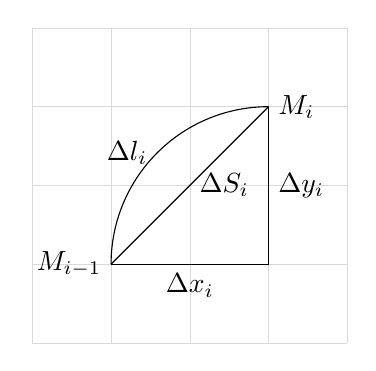
\begin{tikzpicture}
  
      \draw[very thin, gray!30, step = 1cm] (0, 0) grid (4, 4);
      \draw (1, 1) -- (3, 1) -- (3, 3);
      \draw (3, 3) arc (90:180:2) node[midway, above, left] {\(\Delta l_{i}\)};
      \draw (1, 1) -- (3, 3) node[midway, below, right] {\(\Delta S_{i}\)};

      \draw node[below] at (2, 1) {\(\Delta x_{i}\)};
      \draw node[right] at (3, 2) {\(\Delta y_{i}\)};
      \draw node[left] at (1, 1) {\(M_{i - 1}\)};
      \draw node[right] at (3, 3) {\(M_{i}\)};
    
    \end{tikzpicture}
  \end{multicols}

  \item Заметим, что \(\dfrac{\Delta y_{i}}{\Delta x_{i}}\) это отношение
  конечных приращений, поэтому можно применить т. Лагранжа:
  \begin{align*}
    \exists \xi_{i} \in [x_{i - 1}, x_{i}] \colon
      \frac{\Delta y_{i}}{\Delta x_{i}} = f'(\xi_{i})
    \\
    \Delta S_{i}
    = \sqrt{1 + y'(\xi_{i})^2} \Delta x_{i}
  \end{align*}
  
  \item Составим предел интегральных сумм и перейдем к интегралу:

  \begin{align*}
    S = \lim_{\substack{n \to \infty \\ \tau \to 0}}
      \sum_{i = 1}^{n} \sqrt{1 + y'(\xi_{i})^2} \Delta x_{i}
    \implies S = \int_{a}^{b} \sqrt{1 + y'(x)^2} \dd x
  \end{align*}
\end{enumerate}

\begin{remark}
  Выражение \(\dd l = \sqrt{1 + y'(x)^2} \dd x\) называется дифференциалом дуги.
\end{remark}
  \question{Решение ЛНУ\(_2\) с постоянными коэффициентами: специальная правая часть, поиск частного решения методом неопределенных коэффициентов.}


  \subsection{%
  Правила дифференцирования: производная сложной функции, инвариантность
  дифференциала.%
}

\begin{theorem}[Производная сложной функции]
  \begin{equation*}
    \begin{rcases}
      g(x) \isdiffd{x} \\
      f(g) \isdiffd{g_0 = g(x)}
    \end{rcases}
    \implies
    f'(g(x)) = f'(g) \cdot g'(x)
  \end{equation*}
\end{theorem}

\begin{proof}
  По критерию дифференцируемости имеем

  \begin{equation*} \label{eq:diff-cpx-func-1} \tag{1}
    \begin{aligned}
      u = g(x) \isdiffd{x}
      \implies
      \Delta u = g'(x) \Delta x + \smallo(\Delta x)
    \\
      y = f(g) \isdiffd{g_0}
      \implies
      \Delta y = f'(u) \Delta u + \smallo(\Delta u)
    \\
      \Delta y = f'(u)(g'(x) \Delta x + \smallo(\Delta x)) + \smallo(\Delta u)
    \end{aligned}
  \end{equation*}
  
  Также заметим, что 

  \begin{equation*} \label{eq:diff-cpx-func-2} \tag{2}
    u = g(x) \isdiffd{x} \implies g(x) \iscontd{x}
    \iff
    \Delta x \to 0 \implies \Delta u \to 0
  \end{equation*}

  Напишем определение производной для исходной функции.

  \begin{equation*} \label{eq:diff-cpx-func-3} \tag{3}
    \prh{f(g(x))}'
    = \lim_{\Delta x \to 0} \frac{\Delta y}{\Delta x}
    = \lim_{\Delta x \to 0} f'(u) g'(x)
      + f'(u) \frac{\smallo(\Delta x)}{\Delta x}
      + \frac{\smallo(\Delta u)}{\Delta x}
  \end{equation*}

  Второе и третье слагаемые в дают ноль в пределе, как отношение б.м. функции
  более высокого порядка и её аргумента (см. \eqref{eq:diff-cpx-func-2}), значит
  \(\prh{f(g(x)}' = f'(g) g'(x)\).
\end{proof}

\begin{remark}
  Если необходимо взять производную от композиции нескольких функций, то можно
  пользоваться \quote{расширенной} формулой производной композиции функций
  (правилом цепочки).

  \begin{equation*}
    \prh{f(g(h(\phi(x))))}' = f'(g) \cdot g'(h) \cdot h'(\phi) \cdot \phi'(x)
  \end{equation*}
\end{remark}

\begin{theorem}
  Первый дифференциал сохраняет инвариантность формы.
\end{theorem}

\begin{proof}
  Рассмотрим \(y = f(x)\), пусть \(x = u(t)\). Используя определение
  дифференциала и производную сложной функции получаем

  \begin{equation*}
    \dd y
    = y'_t \dd t
    = y'_x \cdot \under{x'_t \dd t}{\dd x}
    = y'_x \dd x
  \end{equation*}
  
  Таким образом, форма дифференциала не зависит от того, является аргумент
  функции независимой переменной или функцией другого аргумента.
\end{proof}

\begin{theorem}[Производная обратной функции]
  \begin{equation*}
    \begin{rcases}
      f(x) \isdiffd{x_0} \\
      f'(x_0) \neq 0 \\
      \exists g(y) = f^{-1}(y)
    \end{rcases}
    \implies
    g'(y) = \frac{1}{f'(x)}
  \end{equation*}
\end{theorem}

\begin{proof}
  Раскроем производную по определению и преобразуем.

  \begin{equation*} \label{eq:diff-inv-func-1} \tag{1}
    f'(x) = \lim_{\Delta x \to 0} \frac{\Delta y}{\Delta x}
    = \frac{1}{\lim_{\Delta x \to 0} \frac{\Delta x}{\Delta y}}
  \end{equation*}

  Заметим, что

  \begin{equation*} \label{eq:diff-inv-func-2} \tag{2}
    \begin{aligned}
      f(x) \isdiffd{x_0}
      \implies f(x) \iscontd{x_0}
      \iff \Delta x \to 0 \implies \Delta y \to 0
    \\
      \frac{1}{\lim_{\Delta x \to 0} \frac{\Delta x}{\Delta y}}
      = \frac{1}{\lim_{\Delta y \to 0} \frac{\Delta x}{\Delta y}}
    \end{aligned}
  \end{equation*}

  Выражение в знаменателе это и есть производная обратной функции. Таким образом
  из \eqref{eq:diff-inv-func-1} и \eqref{eq:diff-inv-func-2} следует, что

  \begin{equation*}
    f'(x)
    = \frac{1}{\lim_{\Delta y \to 0} \frac{\Delta x}{\Delta y}}
    = \frac{1}{g'(y)}
    \implies \prh{f^{-1}(y)}' = \frac{1}{f'(x)}
  \end{equation*}
\end{proof}

\begin{theorem}[Производная параметрически заданной функции]
  \begin{equation*}
    \begin{rcases}
      x = a(t) \isdiffd{t_0} \\
      y = b(t) \isdiffd{t_0} \\
      \exists a^{-1}(t) \\
      a'(t_0) \neq 0
    \end{rcases}
    \implies
    y'(x) = \frac{b'(t_0)}{a'(t_0)}
  \end{equation*}
\end{theorem}

\begin{proof}
  Т.к. \(a(t)\) обратима, то \(t = A(x)\), тогда по формуле производной сложной
  функции получаем

  \begin{equation*} \label{eq:diff-param-func-1} \tag{1}
    \prh{b(A(x))}'_x = b'_A \cdot A'_x
  \end{equation*}
  
  По формуле производной обратной функции \(\display{A'_x = \frac{1}{x'_A}}\).
  Учитывая, что \(A(x) = t\) и \(b(t) = y\), подставим это в
  \eqref{eq:diff-param-func-1}.

  \begin{equation*} \label{eq:diff-param-func-2} \tag{2}
    b(t)'_x = b'_t \cdot \frac{1}{x'_t} 
    \implies
    y'(x) = \frac{y'_t}{x'_t}
  \end{equation*}
\end{proof}
  \subsection{%
  Производные элементарных функций: константа, степенная функция.%
}

\begin{theorem}
  \begin{equation*}
    f(x) = c \implies f'(x) = 0
  \end{equation*}
\end{theorem}

\begin{proof}
  По определению производной

  \begin{equation*}
    f'(x) = \lim_{\Delta x \to 0} \frac{\Delta y}{\Delta x}
  \end{equation*}

  Т.к. \(f(x) = c\), то \(\Delta y = 0\), а значит

  \begin{equation*}
    f'(x) = \lim_{\Delta x \to 0} \frac{0}{\Delta x} = 0
  \end{equation*}
\end{proof}

\begin{theorem}
  \begin{equation*}
    f(x) = x^n \implies f'(x) = n x^{n - 1}
  \end{equation*}
\end{theorem}

\begin{proof}
  По определению производной
  
  \begin{equation*}
    f'(x)
    = \lim_{\Delta x \to 0} \frac{\Delta y}{\Delta x}
    = \lim_{\Delta x \to 0} \frac{f(x_0 + \Delta x) - f(x_0)}{\Delta x}    
  \end{equation*}

  Воспользуемся биномом Ньютона и вычислим полученную дробь.

  \begin{equation*}
    \begin{aligned}
      \frac{f(x_0 + \Delta x) - f(x_0)}{\Delta x}
    = \\
      \frac{(x_0 + \Delta x)^n - x_0^n}{\Delta x}
    = \\
      \frac{x_0^n + n x_0^{n - 1} \Delta x + \dotsc + (\Delta x)^n -
        x_0^n}{\Delta x}
    = \\
      \frac{n x_0^{n - 1} \Delta x + \dotsc + (\Delta x)^n}{\Delta x}
    = \\
      n x_0^{n - 1} + \dotsc + (\Delta x)^{n - 1}
    \end{aligned}
  \end{equation*}

  Заметим, что все слагаемые, кроме первого содержат \(\Delta x\), причем мы
  рассматриваем предел при \(\Delta x \to 0\). Это значит, что в пределе все
  слагаемые кроме первого обнулятся и получится

  \begin{equation*}
    f'(x)
    = \lim_{\Delta x \to 0} (n x_0^{n - 1} + \dotsc + (\Delta x)^{n - 1})
    = n x_0^{n - 1}
  \end{equation*}
\end{proof}

  \subsection{%
  Преобразование базиса и координат.%
}

\subheader{Переход к новому базису}

Пусть есть старый базис \(\set{\basis_i}_{i = 1}^n\) и новый базис
\(\set{\basis’_i}_{i = 1}^n\) и необходимо перейти от старого базиса к новому.
Разложим каждый из векторов старого базиса по новому базису.

\begin{equation*}
  \begin{cases}
    \basis_1 & = a_{1, 1} \basis'_1 + \dotsc + a_{1, n} \basis'_n \\
    \vdots & \\
    \basis_n & = a_{n, 1} \basis'_1 + \dotsc +  a_{n, n} \basis'_n 
  \end{cases}  
\end{equation*}

Теперь рассмотрим разложение произвольного вектора \(x\) в старом базисе.
Заменим в этом разложении каждый из векторов старого базиса на его разложение по
новому базису, перегруппируем и получим

\begin{equation*}
  \begin{aligned}
    x & = b_1 \basis_1 + \dotsc + b_n \basis_n  
  \\
    x & = b_1 (a_{1, 1} \basis'_1 + \dotsc + a_{1, n} \basis'_n)
      + \dotsc
      + b_n (a_{n, 1} \basis'_1 + \dotsc + a_{n, n} \basis'_n)
  \\
    x & = (b_1 a_{1, 1} + \dotsс + b_n a_{n, 1}) \basis'_1
    + \dotsc
    + (b_1 a_{1, n} + \dotsc + b_n a_{n, n}) \basis'_n
  \end{aligned}
\end{equation*}

\begin{remark}
  В матричном виде переход к новому базису можно выразить так

  \begin{equation*}
    B' = A^{-1 }B
  \end{equation*}

  А новые координаты можно вычислить так

  \begin{equation*}
    X_{B'} = A^T X_B
  \end{equation*}
\end{remark}

\subheader{Преобразования системы координат (СК)}

В качестве преобразований СК будет рассматривать только движения, причем будем
рассматривать движения именно СК, а не фигуры.

\begin{definition}
  Движение это отображение пространства в себя, которые сохраняет расстояние
  между точками.

  \begin{equation*}
    \begin{aligned}
      M(x, y) & \rarr{f} M'(x', y')
    \\
      O & \rarr{f} O'
    \\
      \abs{\vec{OM}} & = \abs{\vec{O'M'}}
    \end{aligned}
  \end{equation*}
\end{definition}

Существует несколько типов движений.

\begin{enumerate}
\item
  Осевая симметрия.
\item
  Параллельный перенос (сдвиг).
\item
  Поворот относительно точки.
\end{enumerate}

\subheader{Осевая симметрия}

\begin{definition}
  Осевой симметрией называется симметрия относительно одной (или нескольких) из
  осей.
\end{definition}

Координаты при этом меняются следующим образом.

\begin{equation*}
  \begin{array}{cc}
    \text{Симметрия относительно \(OY\)}
    &
    \text{Симметрия относительно \(OX\)}
  \\
    \begin{cases}
      x' = -x \\
      y' = y
    \end{cases}
    &
    \begin{cases}
      x' = x \\
      y' = -y
    \end{cases}
  \end{array}
\end{equation*}

\subheader{Параллельный перенос}

При параллельном переносе СК на вектор \(\vec{OO'}\) каждая точка переносится на
этот вектор. Перенос обозначается \(P_{\vec{a}}\), где \(\vec{a}\) это вектор
переноса.  

Координаты при этом меняются следующим образом:

\begin{equation*}
  \begin{cases}
    x = x' + x_0 \\
    y = y' + y_0
  \end{cases}
  \qquad
  \begin{cases}
    x' = x - x_0 \\
    y' = y - y_0
  \end{cases} 
\end{equation*}

где \((x_0, y_0)\) координаты точки \(O'\) в старой СК.

\begin{remark}
  При параллельном переносе направления осей сохраняются, т.е.
  \(OX \collinear O'X'\) и \(OY \collinear  O'Y'\).
\end{remark}

\subheader{Поворот СК}

Рассмотрим поворот СК \textbf{вокруг начала координат} на угол \(\alpha\)
\textbf{против часовой стрелки}.

Координаты при этом меняются следующим образом:

\begin{equation*} \label{eq:CS-rotate} \tag{ROT}
  \begin{cases}
    x = x' \cos \alpha - y' \sin \alpha \\
    y = x' \sin \alpha + y' \cos \alpha
  \end{cases}
  \qquad
  \begin{cases}
    x' = x \cos \alpha + y \sin \alpha \\
    y' = -x \sin \alpha + y \cos \alpha
  \end{cases}
\end{equation*}

\begin{remark}
  Матрица \(\display{\mtxp{
    \cos \alpha & -\sin \alpha \\
    \sin \alpha & \cos \alpha
  }}\)  называется матрицей поворота. Если умножить старые координаты на неё, то
  получатся новые координаты. Матрица обратного преобразования является обратной
  матрицей к матрице поворота. 
\end{remark}

\galleryone{01_19_01}{Смена координат при повороте СК}
 
Покажем, как можно получить формулы \eqref{eq:CS-rotate}.

\begin{proof}
  При повороте центр СК остается прежним и угол между осями не изменяется,
  значит \(O' = O\) и \(\angle(OX, OY) = \angle(OX', OY')\). Пусть
  \(\abs{\vec{a}} = \rho\), введём полярную СК (\(O\) полюс, \(OX\) полярная
  ось). Обозначим \((x, y)\) координаты вектора \(\vec{a}\) в старой СК, а
  \((x', y')\)~--- в новой. Из \figref{01_19_01} получаем

  \begin{align*}
    \begin{cases}
      x' = OB = \rho \cos (\omega - \alpha) \\
      y' = OA = \rho \sin(\omega - \alpha)
    \end{cases}
    \label{eq:CS-rotate-1} \tag{1}
  \\
    \begin{cases}
      x = OC = \rho \cos \omega \\
      y = OD = \rho \sin \omega
    \end{cases}
    \label{eq:CS-rotate-2} \tag{2}
  \end{align*}

  В \eqref{eq:CS-rotate-1} применим тригонометрические формулы.

  \begin{equation*} \label{eq:CS-rotate-3} \tag{3}
    \begin{cases}
      x' = \under{\rho \cos \omega}{x} \cos \alpha
        + \under{\rho \sin \omega}{y} \sin \alpha
      \\
      y' = \under{\rho \sin \omega}{y} \cos \alpha
        - \under{\rho \cos \omega}{x} \sin \alpha
    \end{cases}
  \end{equation*}

  Подставим \eqref{eq:CS-rotate-2} в \eqref{eq:CS-rotate-3}.

  \begin{equation*}
    \begin{cases}
      x' = x \cos \alpha + y \sin \alpha \\
      y' = y \cos \alpha - x \sin \alpha
    \end{cases}
    \implies
    \begin{cases}
      x' = x \cos\alpha + y \sin \alpha \\
      y' = -x \sin \alpha + y \cos \alpha
    \end{cases}
  \end{equation*}
\end{proof}

  \question{Виды векторных полей и их свойства (теоремы о поле градиента и поле вихря).}


  \question{Механический смысл потока и дивергенции.}


  \question{Признаки сходимости несобственных интегралов: второй признак сравнения (предельный).}


  \subsection{Теоремы о дифференцируемых функциях. Теорема Ферма.}

\end{questions}

\end{document}